\documentclass[12pt]{amsart}

\usepackage{amsmath,amsfonts,amssymb,mathabx,shuffle,latexsym,breqn,stmaryrd,mathtools,mathrsfs}
\usepackage{enumitem}
\usepackage{subcaption}
\usepackage[usenames, dvipsnames]{xcolor}
\usepackage[backref=page]{hyperref}
\usepackage{ytableau}
\usepackage{tikz-cd}
\usepackage{array}
\usepackage{tikz}
\usetikzlibrary{calc, shapes, backgrounds,arrows.meta,positioning,plotmarks,decorations.markings}
\tikzset{>=Straight Barb,
  head/.style = {fill = white, text=black},
  plaque/.style = {draw, rectangle, minimum size = 10mm}, 
  pil/.style={->,thick},
  pilpil/.style={<->,thick},
  junct/.style = {draw,circle,inner sep=0.5pt,outer sep=0pt, fill=black}
  }
 
%\usepackage{fullpage}
\setlength{\evensidemargin}{0in} 
\setlength{\textheight}{8.4in}      
\setlength{\textwidth}{6in}    
\setlength{\topmargin}{0in}      
\setlength{\oddsidemargin}{0in} 

%%%%%%%%%%%%%%%%%%%%%%%%%%%%%
% Dynkin things
\newcommand{\dynkinradius}{.15cm}
\newcommand{\dynkinstep}{.58cm}
\newcommand{\dynkinnormal}[2]{\fill (\dynkinstep*#1,\dynkinstep*#2) circle (\dynkinradius);}
%\newcommand{\dynkinXsize}{1.5}
\newcommand{\dynkinmin}[2]{\filldraw[fill=SkyBlue,draw=black] (\dynkinstep*#1,\dynkinstep*#2) circle (\dynkinradius);}
\newcommand{\dynkinline}[4]{\draw[thin] (\dynkinstep*#1,\dynkinstep*#2) -- (\dynkinstep*#3,\dynkinstep*#4);}
\newcommand{\dynkindots}[4]{\draw[dotted,very thick] (\dynkinstep*#1,\dynkinstep*#2) -- (\dynkinstep*#3,\dynkinstep*#4);}
\newcommand{\dynkindoubleline}[4]{\draw[double,double distance between line centers=0.19em,postaction={decorate}] (\dynkinstep*#1,\dynkinstep*#2) -- (\dynkinstep*#3,\dynkinstep*#4);}

\newenvironment{dynkin}{\begin{tikzpicture}[decoration={markings,mark=at position 0.7 with {\arrow{>[scale=.7]}}}]}
{\end{tikzpicture}}

\usepackage{enumitem}
\newlist{arrowlist}{itemize}{1}
\setlist[arrowlist]{label=$\Rightarrow$}
\newcommand{\x}{\ensuremath{\mathsf{x}}}
\newcommand{\y}{\ensuremath{\mathsf{y}}}
\newcommand{\e}{\ensuremath{\mathsf{e}}}
\newcommand{\aaa}{\ensuremath{\mathsf{a}}}

\newcommand{\gap}{\hspace{1in} \\ \vspace{-.2in}}


%%%%%%%%%%%%%%%%%%%%%%%%%%%%%%%%%%%%%%%%%%%%%%%%%%%%%%%%%%%%
%  Environments 
%%%%%%%%%%%%%%%%%%%%%%%%%%%%%%%%%%%%%%%%%%%%%%%%%%%%%%%%%%%%

\newtheorem{theorem}{Theorem}[section]
\newtheorem{lemma}[theorem]{Lemma}
\newtheorem{proposition}[theorem]{Proposition}
\newtheorem{corollary}[theorem]{Corollary}
\newtheorem{conjecture}[theorem]{Conjecture}

\theoremstyle{definition}
\newtheorem{definition}[theorem]{Definition}
\newtheorem{examplex}[theorem]{Example}
\newenvironment{example}
  {\pushQED{\qed}\renewcommand{\qedsymbol}{$\diamondsuit$}\examplex}
  {\popQED\endexamplex}
\newtheorem{xca}[theorem]{Exercise}
\newtheorem{algorithm}[theorem]{Algorithm}

\theoremstyle{remark}
\newtheorem{remark}[theorem]{Remark}

\numberwithin{equation}{section}


%%%%%%%%%%%%%%%%%%%%%%%%%%%%%%%%%%%%%%%%%%%%%%%%%%%%%%%%%%%%
%  MACROS for this particular document
%%%%%%%%%%%%%%%%%%%%%%%%%%%%%%%%%%%%%%%%%%%%%%%%%%%%%%%%%%%%

\DeclareMathOperator{\codim}{codim}
\DeclareMathOperator{\ex}{ex}
\newcommand{\wt}{\ensuremath{\mathrm{wt}}}
\newcommand{\kwt}{\ensuremath{\mathrm{kwt}}}
\newcommand{\rev}{\ensuremath{\mathrm{rev}}}
\newcommand{\inv}{\ensuremath{\mathrm{inv}}}
\newcommand{\reduct}{\ensuremath{\mathtt{reduct}}}
\newcommand{\Des}{\ensuremath{\mathrm{Des}}}
\newcommand{\SSYT}{\ensuremath{\mathrm{SSYT}}}
\newcommand{\SYT}{\ensuremath{\mathrm{SYT}}}
\newcommand{\sit}{\ensuremath{\mathrm{sit}}}
\newcommand{\gen}{\ensuremath{\mathrm{gen}}}
\renewcommand{\emptyset}{\varnothing}

\newcommand{\inc}{\ensuremath{\mathrm{Inc}}}
\newcommand{\incgl}{\inc_{\mathrm{gl}}}
\newcommand{\pro}{\mathfrak{pro}}
\newcommand{\evac}{\mathfrak{Evac}}
\newcommand{\rot}{\ensuremath{\mathsf{rot}}}
\newcommand{\Frame}{\ensuremath{\mathsf{Frame}}}
\newcommand{\rect}{\ensuremath{\mathsf{rect}}}
\newcommand{\LIS}{\ensuremath{\mathsf{LIS}}}
\newcommand{\swap}{\ensuremath{\mathsf{swap}}}
\newcommand{\ein}{\ensuremath{\mathsf{In}}}
\newcommand{\eout}{\ensuremath{\mathsf{Out}}}
\newcommand{\decr}{\ensuremath{\mathsf{Decr}}}
\newcommand{\partialfill}{\ensuremath{\mathsf{PartialFilling}}}
\newcommand{\bulltab}{\ensuremath{\mathsf{BulletTableaux}}}
\newcommand{\slide}{\ensuremath{\mathsf{slide}}}
\newcommand{\rep}{\ensuremath{\mathsf{Rep}}}
\newcommand{\blank}{\phantom{2}}
\newcommand{\shape}{\ensuremath{\mathsf{sh}}}
\newcommand{\id}{\ensuremath{\mathrm{id}}}
\newcommand{\bbb}{\ensuremath{\mathsf{b}}}
\newcommand{\dist}{\ensuremath{\mathrm{Dist}}}
\newcommand{\rank}{\ensuremath{\mathrm{rk}}}
\newcommand{\mot}{\ensuremath{\mathsf{Mot}}}
\newcommand{\pp}{\ensuremath{\mathsf{PP}}}
\newcommand{\deflate}{\ensuremath{\mathsf{Defl}}}
\newcommand{\inflate}{\ensuremath{\mathsf{VecInfl}}}
\newcommand{\reinflate}{\ensuremath{\mathsf{Reinfl}}}
\newcommand{\tinflate}{\ensuremath{\mathsf{Infl}}}
\newcommand{\content}{\ensuremath{\mathsf{Con}}}
\newcommand{\compress}{\ensuremath{\mathsf{DeflCon}}}

\newcommand{\uu}{\mathcal{I}}

% Fancy comments
\usepackage[colorinlistoftodos]{todonotes}
\newcommand{\holly}[1]{\todo[size=\tiny,color=blue!30]{#1 \\ \hfill --- Holly}}
\newcommand{\Holly}[1]{\todo[size=\tiny,inline,color=blue!30]{#1
      \\ \hfill --- Holly}}
\newcommand{\oliver}[1]{\todo[size=\tiny,color=red!30]{#1 \\ \hfill --- Oliver}}
\newcommand{\Oliver}[1]{\todo[size=\tiny,inline,color=red!30]{#1
      \\ \hfill --- Oliver}}

\begin{document}

%%%%%%%%%%%%%%%%%%%%%%%%%%%%%%%%%%%%%%%%%%%%%%%%%%%%%%%%%%%%
%  TITLE PAGE information
%%%%%%%%%%%%%%%%%%%%%%%%%%%%%%%%%%%%%%%%%%%%%%%%%%%%%%%%%%%%

%     [Short Title]{Full Title}
\title[Orbits of plane partitions]{Orbits of plane partitions of exceptional Lie type}  

%    Information for first author
\author[H. Mandel]{Holly Mandel}
\address[HM]{Department of Mathematics, University of California, Berkeley, \linebreak Berkeley, CA 94720}
\email{holly.mandel@berkeley.edu}
%\thanks{}

\author[O. Pechenik]{Oliver Pechenik}
\address[OP]{Department of Mathematics, University of Michigan, Ann Arbor, MI 48109}
\email{pechenik@umich.edu}
%\thanks{}

%    General info
\subjclass[2010]{Primary 05A15; Secondary 05E18, 06A07, 17B25}

\date{\today}

%\dedicatory{}

\keywords{plane partition, increasing tableau, promotion, rowmotion, exceptional Lie algebra, minuscule poset, cyclic sieving phenomenon}


\begin{abstract}
For each minuscule flag variety $X$, there is a corresponding minuscule poset, describing its Schubert decomposition. We study an action on plane partitions over such posets, introduced by P.~Cameron and D.~Fon-der-Flaass (1995).
For plane partitions of height at most $2$, D.~Rush and X.~Shi (2013) proved an instance of the cyclic sieving phenomenon, completely describing the orbit structure of this action. They noted their result does not extend to greater heights in general; however, when $X$ is one of the two minuscule flag varieties of exceptional Lie type $E$, they conjectured explicit instances of cyclic sieving for all heights.

We prove their conjecture in the case that $X$ is the Cayley-Moufang plane of type $E_6$. For the other exceptional minuscule flag variety, the Freudenthal variety of type $E_7$, we establish their conjecture for heights at most $4$, but show that it fails generally. We further give a new proof of a unpublished cyclic sieving of D.~Rush and X.~Shi (2011) for plane partitions of any height in the case $X$ is an even-dimensional quadric hypersurface. 
Our argument uses ideas of K.~Dilks, O.~Pechenik, and J.~Striker (2017) to relate the action on plane partitions to combinatorics derived from $K$-theoretic Schubert calculus. 
\end{abstract}

\maketitle
%\tableofcontents


%%%%%%%%%%%%%%%%%%%%%%%%%%%%%%%%%%%%%%%%%%%%%%%%%%%%%%%%%%%%%%%%
%
\section{Introduction}
%
%%%%%%%%%%%%%%%%%%%%%%%%%%%%%%%%%%%%%%%%%%%%%%%%%%%%%%%%%%%%%%%%
\label{sec:introduction}

The \emph{minuscule posets} are a remarkable collection of partially-ordered sets that arise naturally from the representation theory of Lie algebras or alternatively from the Schubert calculus of certain generalized flag varieties. We study dynamic enumerative properties of plane partitions over these posets.

A special case of this situation is that of ordinary plane partitions fitting inside a fixed rectangular box. In this context, P.~Cameron and D.~Fon-der-Flaass \cite{Cameron.Fonderflaass} initiated the study of a combinatorially-natural operator $\Psi$. This operator is now generally known as \emph{rowmotion} and has become a subject of intense study (cf., e.g., \cite{Panyushev,Striker.Williams,Armstrong.Stump.Thomas,Rush.Shi,Einstein.Propp,Propp.Roby,Grinberg.Roby:2,Grinberg.Roby:1,DPS,Vorland}).
We will define and describe in detail both minuscule posets and the operation of rowmotion in Sections~\ref{sec:minuscule} and \ref{sec:rowmotion}, respectively.

For any poset $P$, let $\pp^k(P)$ denote the set of plane partitions of height at most $k$ over $P$, that is to say the set of order ideals in the product $P \times {\bf k}$ of $P$ with a chain poset of size $k$. Let $f_P^k$ denote the generating function that enumerates the elements of $\pp^k(P)$  by cardinality. In the special case $k \leq 2$ and $P$ minuscule, D.~Rush and X.~Shi \cite{Rush.Shi} showed that $f_P^k$ also encodes the orbit structure of rowmotion via an instance of the {\bf cyclic sieving phenomenon} (introduced by V.~Reiner, D.~Stanton, and D.~White \cite{Reiner.Stanton.White}). That is to say that for $k \leq 2$, the number of minuscule plane partitions fixed by the $d$-fold application of rowmotion $\Psi^{\circ d}$ is the evaluation of the polynomial $f_P^k$ at $\zeta^d$, where $\zeta$ is any primitive $n$th root-of-unity and $n$ is the order of $\Psi$ on $\pp^k(P)$. (Since some of our other operators have superscripts in their names, we will consistently denote $d$-fold composition of any operator $\tau$ by $\tau^{\circ d}$, instead of the more usual notation $\tau^d$, which could otherwise be ambiguous.)

It was noted, however, in \cite{Rush.Shi} that this instance of cyclic sieving does not extend to the case $k\geq 3$ for general minuscule posets.
Nonetheless, D.~Rush and X.~Shi conjectured the following. (The minuscule posets in question are illustrated in Figure~\ref{fig:min_poset_E}.)
\begin{conjecture}[{\cite[Conjecture~11.1]{Rush.Shi}}]\label{conj:rush.shi}
Let $P$ be one of the two minuscule posets associated to an exceptional Lie algebra of type $E$ and let $k \in \mathbb{Z}_{\geq 0}$. Then $f_P^k$ is a cyclic sieving polynomial for the action of $\Psi$ on $\pp^k(P)$.
\end{conjecture}

\begin{figure}[h]
	\begin{subfigure}[b]{0.35\textwidth}
		\centering
		\ydiagram{3+5,3+3,2+3,5}
		\caption{Cayley-Moufang poset}
	\end{subfigure} \\ \vspace{4mm}
	\begin{subfigure}[b]{0.35\textwidth}
		\centering
		\ydiagram{8+1,8+1,8+1,7+2,4+5,4+5,4+3,3+3,6}
		\caption{Freudenthal poset}
	\end{subfigure}
\caption{The two minuscule posets associated to exceptional Lie algebras of type $E$. Here, we have drawn the posets to resemble Young diagrams in Cartesian (``French'') orientation; the boxes are the elements of the poset and each box covers the box immediately below it and the box immediately to its left (if such boxes exist). Hence the minimal element of each poset is the box at the far left of the bottom row.
 The Cayley-Moufang poset is associated to $E_6$, while the Freudenthal poset is associated to $E_7$. (There is no minuscule poset associated to $E_8$.)}
\label{fig:min_poset_E}
\end{figure}

Our main result is to completely resolve Conjecture~\ref{conj:rush.shi}. 
\begin{theorem}\label{thm:exceptionals}
Conjecture~\ref{conj:rush.shi} holds for the $E_6$ minuscule poset (cf.~Figure~\ref{fig:min_poset_E}A) and all $k$, but holds for the $E_7$ minuscule poset (cf.~Figure~\ref{fig:min_poset_E}B) only when $k \leq 4$. 
\end{theorem}  
Verification of Conjecture~\ref{conj:rush.shi} in the the cases $k \leq 4$ for the $E_6$ minuscule poset and $k \leq 3$ for the $E_7$ minuscule poset was previously reported in \cite{Rush.Shi}. Our new results are therefore:
\begin{itemize}
\item cyclic sieving for the $E_6$ minuscule poset when $k > 4$,
\item cyclic sieving for the $E_7$ minuscule poset when $k = 4$, and
\item failure of the conjectured cyclic sieving for the $E_7$ minuscule poset for $k > 4$.
\end{itemize}

Our approach to proving Theorem~\ref{thm:exceptionals} is to extend the ideas of K.~Dilks, O.~Pechenik, and J.~Striker \cite{DPS} to this minuscule setting, thereby relating the action of $\Psi$ to the action of \emph{$K$-promotion} on \emph{increasing tableaux}. $K$-promotion was first studied in \cite{Pechenik} building on combinatorial tools for $K$-theoretic Schubert calculus due to H.~Thomas and A.~Yong \cite{Thomas.Yong:K}. We show that the action of $K$-promotion is controlled by its behavior on a finite subset of increasing tableaux. By understanding the orbit structure of this subset, we are able to determine the complete orbit structure, thereby establishing Theorem~\ref{thm:exceptionals}.

Having developed these methods, it becomes straightforward to prove the following additional result.
\begin{theorem}\label{thm:propeller}
Let $P$ be a minuscule poset associated to an even-dimensional quadric of type $D$ (cf.~Figure~\ref{fig:min_poset}C) and let $k \in \mathbb{Z}_{\geq 0}$. Then $f_P^k$ is a cyclic sieving polynomial for the action of $\Psi$ on $\pp^k(P)$.
\end{theorem}
Theorem~\ref{thm:propeller} was previously announced by D.~Rush and X.~Shi \cite[Theorem~10.1]{Rush.Shi}; however, they omitted their lengthy proof \cite[\textsection 10]{Rush.Shi:report} from the published paper. We believe that our alternative proof of Theorem~\ref{thm:propeller} via $K$-theoretic combinatorics provides a different understanding.

Often instances of the cyclic sieving phenomenon can be proven using representation-theoretic techniques \cite{Reiner.Stanton.White, Rhoades:thesis}, and when instances are established in a more direct fashion (as we do here), it may be a clue toward as yet undeveloped algebra (cf.\ \cite{Rhoades:skein}). The results in Theorems~\ref{thm:exceptionals} and \ref{thm:propeller} perhaps suggest the existence of new symmetric group module structures on the sets $\pp^k(P)$; however, we do not currently understand how to build such structures with the requisite properties in these cases.

This paper is organized as follows. In Section~\ref{sec:minuscule}, we define the minuscule posets, recalling their classification and certain other properties we will use. In Section~\ref{sec:rowmotion}, we collect the facts we need about the rowmotion operator $\Psi$. Section~\ref{sec:Kpromotion} concerns the operation of $K$-promotion on increasing tableaux, the key tool in our proofs of Theorems~\ref{thm:exceptionals} and \ref{thm:propeller}. In Section~\ref{sec:equivariant}, we demonstrate the equivariant bijection between $\pp^k(P)$ under the action of $\Psi$ and certain increasing tableaux under $K$-promotion, extending the main observation of \cite{DPS}.
Finally, Section~\ref{sec:arithmetic} is devoted to study of these increasing tableaux; our results in this last section prove Theorems~\ref{thm:exceptionals} and \ref{thm:propeller} via the equivariant bijection of Section~\ref{sec:equivariant}.

\section{Minuscule posets}\label{sec:minuscule}

Let ${\sf G}$ be a complex connected reductive Lie group with maximal torus ${\sf T}$. Denote by $W$ the Weyl group $N_{\sf G}({\sf T})/{\sf T}$. The root system $\Phi$ of ${\sf G}$ may be partitioned $\Phi^+ \sqcup \Phi^-$ into positive and negative roots according to a choice $\Delta$ of simple roots. There is a natural poset structure on $\Phi^+$ obtained as the transitive closure of the covering relation $\alpha \lessdot \beta$ if and only if $\beta - \alpha \in \Delta$. The choice of bipartition of $\Phi$ into positive and negative roots further specifies a choice of a Borel subgroup ${\sf B}_+ \subset {\sf G}$ and an opposite Borel subgroup ${\sf B}_- \subset {\sf G}$ with ${\sf B}_+ \cap {\sf B}_- = {\sf T}$.

We say $\delta \in \Delta$ is {\bf minuscule} if for every $\alpha \in \Phi^+$, $\delta^\vee$ appears with multiplicity at most $1$ in the simple coroot expansion of $\alpha^\vee$. The classification of minuscule roots is well known and is illustrated in Figure~\ref{fig:minuscule} in terms of Dynkin diagrams.

\begin{figure}[h]
 \renewcommand*{\arraystretch}{1.6}
\begin{tabular}{|>{$}r<{$}m{3.2cm}|}
\hline
A_n &
  \begin{dynkin}
    \dynkinline{1}{0}{3}{0};
    \dynkindots{3}{0}{4}{0};
    \dynkinline{4}{0}{6}{0};
    \foreach \x in {1,...,6}
    {\dynkinmin{\x}{0}}
  \end{dynkin}
 \\  \hline B_n &
  \begin{dynkin}
    \dynkinline{1}{0}{2}{0};
    \dynkindots{2}{0}{3}{0};
    \dynkinline{3}{0}{4}{0};
    \dynkindoubleline{4}{0}{5}{0};
    \dynkinmin{5}{0};
    \foreach \x in {1,...,4}
    {
        \dynkinnormal{\x}{0}
    }
  \end{dynkin}
\\ \hline   C_n 
&
  \begin{dynkin}
    \dynkinline{1}{0}{2}{0};
    \dynkindots{2}{0}{3}{0};
    \dynkinline{3}{0}{4}{0};
    \dynkindoubleline{5}{0}{4}{0};
    \dynkinmin{1}{0};
    \foreach \x in {2,...,5}
    {
        \dynkinnormal{\x}{0}
    }
  \end{dynkin}
\\ \hline 
D_n
&
  \begin{dynkin}
    \foreach \x in {2,...,4}
    {
        \dynkinnormal{\x}{0}
    }
        \dynkinline{3}{0}{4}{0}
    \dynkinline{4}{0}{4.5}{.9}
    \dynkinline{4}{0}{4.5}{-.9}
        \dynkinline{1}{0}{2}{0}
    \dynkinmin{4.5}{.9}
    \dynkinmin{4.5}{-.9}
        \dynkinmin{1}{0}
    \dynkindots{2}{0}{3}{0}
  \end{dynkin} 
\\  \hline  E_6 
&
  \begin{dynkin}
    \foreach \x in {2,...,4}
    {
        \dynkinnormal{\x}{0}
    }
        \dynkinline{1}{0}{5}{0}
    \dynkinline{3}{0}{3}{1}
    \dynkinmin{1}{0}
    \dynkinmin{5}{0}
    \dynkinnormal{3}{1}
  \end{dynkin}
\\    E_7
&
  \begin{dynkin}
    \foreach \x in {1,...,5}
    {
        \dynkinnormal{\x}{0}
    }
        \dynkinline{1}{0}{6}{0}
    \dynkinline{3}{0}{3}{1}
    \dynkinmin{6}{0}
    \dynkinnormal{3}{1}
  \end{dynkin} \\
  \hline
\end{tabular}
 \caption{In each of the finite-type Dynkin diagrams above, each minuscule root is marked as a pale blue circle, while the non-minuscule simple roots are marked in black. In type $A_n$, every node is minuscule, while in the other types only the indicated leaves are minuscule. The remaining finite-type Dynkin diagrams are omitted as they have no minuscule nodes.}\label{fig:minuscule}
\end{figure}

For each minuscule simple root $\delta$, there is an associated {\bf minuscule poset} $P_\delta$ obtained as the subposet of $\Phi^+$ induced on those positive roots $\alpha$ where $\delta$ appears with nonzero coefficient in the simple root expansion of $\alpha$. 

Alternatively, one may obtain the minuscule posets via the geometry of certain generalized flag varieties. If ${\sf P}_\delta \supset {\sf B_+}$ denotes the maximal parabolic subgroup of ${\sf G}$ associated to the minuscule simple root $\delta$, then the space $X = {\sf G} / {\sf P}_\delta$ is called a {\bf minuscule variety}. The minuscule varieties are smooth projective varieties with various nice geometric properties (cf.,~e.g.,~\cite{Billey.Lakshmibai} for details). The natural action of the Borel subgroup ${\sf B}_+$ on $X$ has finitely-many orbits, whose Zariski closures are the {\bf Schubert varieties}. Given two Schubert varieties in $X$, it is known that they are either disjoint or else one is a subset of the other. Indeed the poset $Y_X$ of Schubert varieties of $X$ with respect to inclusion is a distributive lattice and its corresponding poset of join irreducibles is isomorphic to the minuscule poset $P_\delta$ for the minuscule simple root $\delta$, as constructed above.

The minuscule posets are completely classified. We illustrate them here in Figures~\ref{fig:min_poset_E} and \ref{fig:min_poset}. Our focus will be on the {\bf propellers}, the {\bf Cayley-Moufang poset}, and the {\bf Freudenthal poset} as shown in Figures~\ref{fig:min_poset}C, \ref{fig:min_poset_E}A, and \ref{fig:min_poset_E}B, respectively. The propeller with $k$ elements ($k \geq 6$) is associated to the minuscule node that is not adjacent to the trivalent node in the $D_{\frac{k+2}{2}}$ Dynkin diagram, the Cayley-Moufang poset is associated to the unique minuscule simple root for $E_6$, and the Freudenthal poset is associated to the unique minuscule simple root for $E_7$ (cf.\ Figure~\ref{fig:minuscule}). The corresponding minuscule varieties are, respectively, even-dimensional quadric hypersurfaces, the octonionic projective plane (or Cayley-Moufang plane), and the Freudenthal variety. The remaining minuscule roots yield minuscule posets that are \emph{rectangles} or \emph{shifted staircases} (illustrated in Figure~\ref{fig:min_poset}A and B). These correspond respectively to type $A$ Grassmannians and to maximal orthogonal Grassmannians; we will not study these posets further in this paper.

A poset that is linearly ordered is called a {\bf chain}; we denote the chain of size $k$ by $\mathbf{k}$. By a {\bf plane partition} of height at most $k$ over a poset $P$, we mean an order ideal of the product poset $P \times \mathbf{k}$.  Clearly, a such a plane partition may be identified with a weakly order-reversing map $\pi : P \to \mathbf{k}$ (i.e., a map $\pi$ such that $p \leq p'$ implies $\pi(p) \geq \pi(p')$). The poset $P$ is called {\bf Gaussian} if the generating function $f_P^k$ enumerating plane partitions of height at most $k$ over $P$ according to cardinality may be expressed in the form
\[
\frac{(1 - x^{h_1 + m})(1 - x^{h_2 + m})\cdots(1 - x^{h_t + m})}{(1 - x^{h_1})(1 - x^{h_2})\cdots(1 - x^{h_t})},
\]
for some nonnegative integers $t, h_1, h_2, \dots, h_t \in \mathbb{Z}_{\geq 0}$ independent of $k$.
R.~Proctor showed that every minuscule poset is Gaussian \cite{Proctor}. Indeed, it is conjectured that there are no other Gaussian posets. Given the beautiful form of these generating functions, it is perhaps not too surprising that $f_P^k$ should in some instances play a role in cyclic sieving phenomena, as in Theorems~\ref{thm:exceptionals} and \ref{thm:propeller}.

\begin{figure}[h]
	\begin{subfigure}[b]{0.27\textwidth}
		\centering
		\ydiagram{4,4,4}
		\caption{Rectangle}
	\end{subfigure}
	\hspace{2cm}
	\begin{subfigure}[b]{0.27\textwidth}
		\centering
		\ydiagram{3+1,2+2,1+3,4}
		\caption{Shifted staircase}
	\end{subfigure} \\
	\vspace{3mm}
	\begin{subfigure}[b]{0.27\textwidth}
		\centering
		\ydiagram{3+5,5}
		\caption{Propeller}
	\end{subfigure}
\caption{Together with the two posets shown in Figure~\ref{fig:min_poset_E}, these are exemplars of all five families of minuscule poset, shown in Cartesian orientation. The elements of each poset are the boxes, and each box is covered by any box immediately above it or immediately to its right. Rectangles may have arbitrary height and width. Shifted staircases have arbitrary width, and height equal to their width. Propellers consist of two rows of arbitrary but equal length, overlapping by two boxes in the center. The Cayley-Moufang and Freudenthal posets of Figure~\ref{fig:min_poset_E} are exceptional, forming singleton families.}\label{fig:min_poset}
\end{figure}

\section{The rowmotion operator $\Psi$}\label{sec:rowmotion}

If $P$ is any poset, let $J(P)$ denote the set of all its order ideals. For $\uu \in J(P)$ an order ideal of $P$, we define $\Psi(\uu) \in J(P)$ to be the order ideal generated by the minimal elements of the complement $P - \uu$. This operator $\Psi$ is closely related to that described in \cite{Brouwer.Schrijver,Duchet,Cameron.Fonderflaass} in slightly different contexts. It was first considered as an action on order ideals by J.~Striker and N.~Williams \cite{Striker.Williams}; we follow them in referring to $\Psi$ as {\bf rowmotion}.

Here, we recall the facts that we will need about rowmotion. For $x \in P$, define the {\bf toggle at $x$} to be the operator $t_x : J(P) \to J(P)$ defined by
\[
t_x(\uu) = \left\{ \begin{array}{ll}
        \uu \cup \{x\}, & \text{for } x \notin \uu \text{ and } \uu \cup \{x\} \in J(P); \\
        \uu - \{x\}, & \text{for } x \in \uu \text{ and } \uu - \{x\} \in J(P);\\
        \uu, & \text{otherwise. }
        \end{array} \right.
\]
Following the terminology of \cite{DPS}, a {\bf $3$-dimensional lattice projection} of a finite ranked poset P is an order- and rank-preserving map $\pi : P \to \mathbb{Z}^3$, where the partial order on $\mathbb{Z}^3$ is given by componentwise comparison and $\mathbb{Z}^3$ is ranked by the sum of the coordinates. Considering the classification of minuscule posets in Figures~\ref{fig:min_poset_E} and \ref{fig:min_poset}, observe that for every minuscule $P$ and any $k > 0$, the poset $P \times {\bf k}$ has an injective $3$-dimensional lattice projection induced from the obvious embeddings of those pictures in the planar lattice. For $v = \{\pm 1 \}^3$ and $i \in \mathbb{Z}$, let 
\begin{equation}\label{eq:taudef}
\tau_{\pi,v}^i = \prod_{\langle v, \pi(x) \rangle = i} t_x.
\end{equation}
That is, $\tau_{\pi,v}^i$ is the composition of the toggles $t_x$ for all $x$ with $\pi(x)$ lying on the affine plane defined by $\langle v, \cdot \rangle = i$. Since the toggles $t_{x_1}$ and $t_{x_2}$ clearly commute whenever neither $x_1$ nor $x_2$ covers the other, this composition is well-defined. Then {\bf  $(\pi, v)$-motion} on $P$ is the operator
\[
\mot_{\pi, v} \coloneqq \prod_{i \in \mathbb{Z}} \tau_{\pi,v}^i,
\]
where the factors are taken in reverse of the natural order. Note that in this product, only finitely many factors act nontrivially, since $\pi(P)$ intersects only a finite number of the affine planes defined by $\langle v, \cdot \rangle = i$. We recall the following pair of results, which are fundamental to our further analysis of rowmotion on minuscule plane partitions.

\begin{proposition}[{\cite[Lemma~1]{Cameron.Fonderflaass}}; {\cite[Proposition~3.18]{DPS}}]
\label{prop:psi_is_toggle}
For any finite ranked poset $P$ with a $3$-dimensional lattice projection $\pi$, we have 
\[
 \Psi  = \mot_{\pi, (1,1,1)}  \] 
 as operators on $J(P)$. \qed
\end{proposition}

\begin{proposition}[{\cite[Theorem~3.25]{DPS}}]
\label{prop:conjugate_actions}
For any finite ranked poset $P$ with a $3$-dimensional lattice projection $\pi$ and any vectors $v,w \in \{ \pm 1 \}^3$, there is an equivariant bijection between $J(P)$ under $\mot_{\pi, v}$ and $J(P)$ under $\mot_{\pi,w}$. In particular, $\mot_{\pi, v}$ and $\mot_{\pi,w}$ induce the same multiset of orbit cardinalities on $J(P)$. \qed
\end{proposition}

\section{$K$-promotion of increasing tableaux}\label{sec:Kpromotion}

\subsection{Definitions}\label{sec:Kpro_defs}
A classical approach to the cohomological Schubert calculus of complex type $A$ Grassmannians is to use the jeu de taquin on standard Young tableaux introduced by M.-P.~Sch\"utzenberger \cite{Schutzenberger:jdt}. (See \cite{Fulton, Manivel} for modern expositions of the classical jeu de taquin theory.) A theme of modern Schubert calculus has been extending such theories to richer generalized cohomologies and in particular into the $K$-theory ring of algebraic vector bundles. For a partial survey of recent work related to $K$-theoretic Schubert calculus and the associated combinatorics, see \cite{Pechenik.Yong:genomic}.

The first $K$-theoretic Littlewood-Richardson rule was discovered by A.~Buch \cite{Buch}; this rule, however, was not based on jeu de taquin. H.~Thomas and A.~Yong \cite{Thomas.Yong:K} later found a different Littlewood-Richardson rule for the same structure coefficients by directly extending M.-P.~Sch\"utzenberger's jeu de taquin. This latter rule was conjectured in \cite{Thomas.Yong:K} to extend to the $K$-theoretic Schubert structure coefficients of all minuscule varieties, as was proven by a combination of \cite{Buch.Ravikumar,Clifford.Thomas.Yong,Buch.Samuel}. In this Thomas-Yong theory, the role of standard Young tableaux is filled by \emph{increasing tableaux}.

\begin{definition}
Let $\lambda$ be an order ideal in a minuscule poset, considered as an generalized Young diagram in Cartesian orientation as in Figures~\ref{fig:min_poset_E} and \ref{fig:min_poset}. An {\bf increasing tableau} of shape $\lambda$ is an assignment of a positive integer to each box of $\lambda$, such that entries strictly increase from left to right along rows and strictly increase from bottom to top going up columns. Let $\inc^q(\lambda)$ denote the set of all increasing tableaux of shape $\lambda$ with all entries at most $q$. We identify $\inc^q(\lambda)$ with the set of all strictly order-preserving maps from the poset $\lambda$ to the chain poset $\mathbf{q}$ of size $q$. For examples of increasing tableaux, see Figures~\ref{fig:kbk} and ~\ref{fig:promotion}.
\end{definition}

Using the $K$-jeu de taquin of H.~Thomas and A.~Yong \cite{Thomas.Yong:K}, one has a $K$-promotion operator $\pro^q$ on $\inc^q(\lambda)$, directly extending M.-P.~Sch\"utzenberger's classical definition of promotion \cite{Schutzenberger:promotion}. $K$-promotion was first studied in \cite{Pechenik}, and has been further investigated in \cite{BPS, Pressey.Stokke.Visentin, Rhoades:skein, DPS, Pechenik:frames,Vorland}. Since studying the action of $\pro^q$ will be fundamental to our proof of Theorems~\ref{thm:exceptionals} and~\ref{thm:propeller}, we must recall the definition of $\pro^q$. 
We will indeed use both the original formulation from \cite{Pechenik}, as well as an equivalent formulation from \cite[Proposition~2.4]{DPS}.

Let $T \in \inc^q(\lambda)$. The {\bf $K$-Bender-Knuth operator} $\rho_i$ acts on $T$ by swapping the letters $i$ and $i+1$ everywhere in $T$ \emph{where doing so would not violate the increasingness conditions.} More precisely, $\rho_i$ looks at the set of boxes labeled $i$ or $i+1$, decomposes that set into edge-connected components, swaps the labels $i$ and $i+1$ in each component that is a single box, and acts trivially on each non-trivial connected component. 
Notice that each $\rho_i$ is an involution.
Using the characterization of \cite[Proposition~2.4]{DPS}, {\bf $K$-promotion} may then be defined by
\[
\pro^q(T) \coloneqq \rho_{q-1} \circ \dots \circ \rho_1(T).
\]
Examples of the action of $K$-Bender-Knuth operators are shown in Figure~\ref{fig:kbk}, while an example of the full process of $K$-promotion is shown in Figure~\ref{fig:promotion}. We will relate $K$-Bender-Knuth operators to poset toggles in Section~\ref{sec:equivariant}.

\begin{figure}[h]
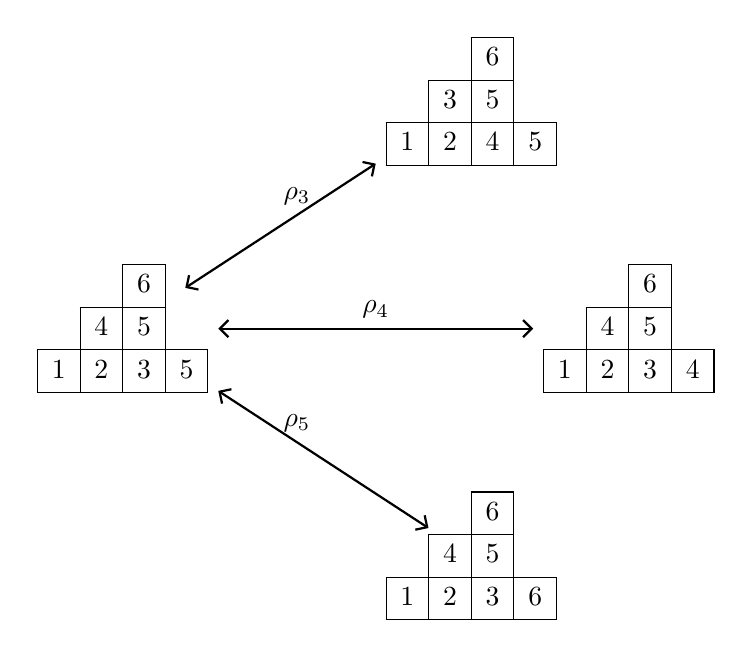
\begin{tikzpicture}
\node (A) {\ytableaushort{\none \none 6,\none 45,1235 } };
\node[above right = 1 and 2 of A] (B) {\ytableaushort{\none \none 6, \none 35, 1245}};
\node[ right = 4 of A] (C) {\ytableaushort{\none \none 6, \none 45,1234}};
\node[below right = 1 and 2 of A] (D) {\ytableaushort{\none \none 6, \none 45,1236}};
\path (A) edge[pilpil,shorten >=-0mm,shorten <=-5mm] node[above]{$\rho_3$} (B);
\path (A) edge[pilpil] node[above]{$\rho_4$} (C);
\path (A) edge[pilpil,shorten >=-8mm] node[above]{$\rho_5$} (D);
\end{tikzpicture}
\caption{The three increasing tableaux on the right are obtained from the increasing tableau at left by applying the indicated $K$-Bender-Knuth operators. The arrows point in both directions since each $K$-Bender-Knuth operator is involutive.}\label{fig:kbk}
\end{figure}

\begin{figure}[h]
\begin{center}
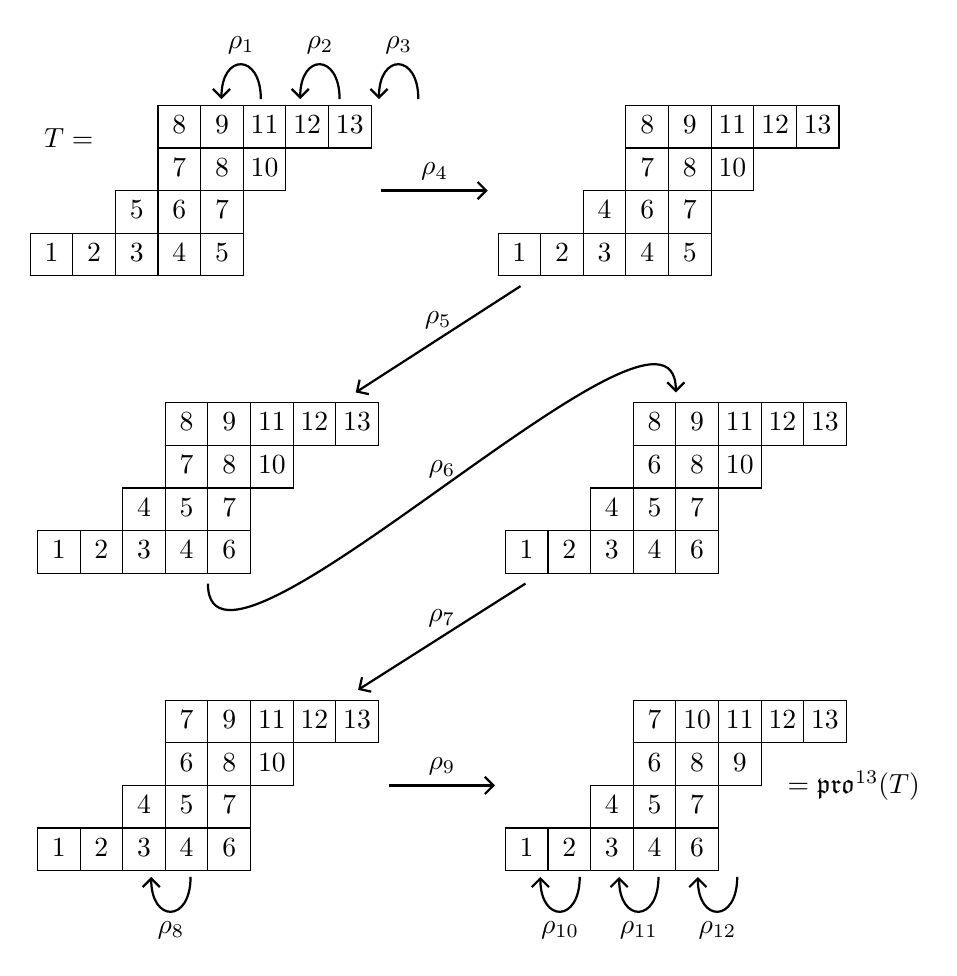
\begin{tikzpicture}
\node (T) {$T= \!\!\!\!\!\!\!$\hspace{-4mm}\ytableaushort{ \none \none \none 89{11}{12}{13},\none \none \none 78{10},\none \none 567, 12345}};
\node[right  = 1.35 of T] (T4) {\ytableaushort{ \none \none \none 89{11}{12}{13}, \none \none \none 78{10}, \none \none 467, 12345}};
\node[below  = 1.35 of T] (T5) {\ytableaushort{   \none \none \none 89{11}{12}{13}, \none \none \none 78{10},\none \none 457,12346}};
\node[right  = 1.35 of T5] (T6) {\ytableaushort{   \none \none \none 89{11}{12}{13}, \none \none \none 68{10},\none \none 457, 12346 }};
\node[below  = 1.35 of T5] (T7) {\ytableaushort{   \none \none \none 79{11}{12}{13},\none \none \none 68{10},\none \none 457, 12346 }};
\node[right  = 1.35 of T7] (T9) {\ytableaushort{  \none \none \none 7{10}{11}{12}{13},\none \none \none 689, \none \none 457, 12346 }};
\node[right = -1 of T9] (finishlabel) {$=\pro^{13}(T)$};
\node[below left = -.3 and -0.7 of T9] (fake1) {};
\node[below left = -.3 and -1.2 of T9] (fake2) {};
\node[below left = -.3 and -1.7 of T9] (fake3) {};
\node[below left = -.3 and -2.2 of T9] (fake4) {};
\node[below left = -.3 and -2.7 of T9] (fake5) {};
\node[below left = -.3 and -3.2 of T9] (fake6) {};
\node[above left = -.3 and -2.5 of T] (fake7) {};
\node[above left = -.3 and -3.0 of T] (fake8) {};
\node[above left = -.3 and -3.5 of T] (fake9) {};
\node[above left = -.3 and -4.0 of T] (fake10) {};
\node[above left = -.3 and -4.5 of T] (fake11) {};
\node[above left = -.3 and -5.0 of T] (fake12) {};
\node[below left = -.3 and -1.7 of T7] (fake13) {};
\node[below left = -.3 and -2.2 of T7] (fake14) {};
\path (T) edge[pil]  node[above]{$\rho_4$} (T4);
\path (T4) edge[pil] node[above]{$\rho_5$} (T5);
\draw[->, thick] (T5.south) .. node[above]{$\rho_6$} controls ([yshift=-3cm] T5) and ([yshift=3cm] T6) .. (T6.north);
\path (T6) edge[pil] node[above]{$\rho_7$} (T7);
\path (fake14) edge[pil,out=270,in=270,looseness=3] node[below]{$\rho_8$} (fake13);
\path (T7) edge[pil] node[above]{$\rho_9$} (T9);
\path (fake2) edge[pil, out=270, in=270, looseness=3] node[below]{$\rho_{10}$} (fake1);
\path (fake4) edge[pil, out=270, in=270, looseness=3] node[below]{$\rho_{11}$} (fake3);
\path (fake6) edge[pil, out=270, in=270, looseness=3] node[below]{$\rho_{12}$} (fake5);
\path (fake8) edge[pil, out=90, in=90, looseness=3] node[above]{$\rho_{1}$} (fake7);
\path (fake10) edge[pil, out=90, in=90, looseness=3] node[above]{$\rho_{2}$} (fake9);
\path (fake12) edge[pil, out=90, in=90, looseness=3] node[above]{$\rho_{3}$} (fake11);
\end{tikzpicture}
\end{center}
\caption{The calculation of the $K$-promotion $\pro^{13}(T)$ of the increasing tableau $T$ (on the Cayley-Moufang poset) through the action of the sequence of $K$-Bender-Knuth operators $\rho_1, \dots, \rho_{12}$.}\label{fig:promotion}
\end{figure}

\subsection{Inflation and deflation}
Suppose $T \in \inc^q(\lambda)$ and consider $T$ as a strictly order-preserving map from $\lambda$ to the chain poset ${\bf q}$. We say that $T$ is {\bf gapless} if this map is surjective; otherwise, $T$ is {\bf gappy}. We write $\incgl^q(\lambda)$ for the subset of all gapless tableaux in $\inc^q(\lambda)$. Notice that the set 
\[
\incgl(\lambda) \coloneqq \bigcup_{q} \incgl^q(\lambda)
\]
is necessarily finite; this fact will be critical for our ability to prove Theorems~\ref{thm:exceptionals} and~\ref{thm:propeller}.

For $T \in \inc^q(\lambda)$, let $N_T \coloneqq |\mathrm{range}(T)|$ be the number of distinct labels in $T$. For each $q$, we define the {\bf deflation} map \[\deflate^q : \inc^q(\lambda) \to \coprod_{0 \leq k \leq q} \incgl^k(\lambda)\] by
\[
[\deflate^q(T)](\x) =
\# \{ h \in \mathrm{range}(T): h \leq T(\x) \} ,
\]
for $T \in \inc^q(\lambda)$ and $\x \in \lambda$. Note that $\deflate^q(T) \in \incgl^{N_T}(\lambda)$ and that $N_T \leq q$.

For positive integers $k \leq j$, let $\binom{[j]}{k}$ denote the collection of binary vectors of length $j$ with $k$ $1$'s. We now define the {\bf content vector} function 
\[
 \content^q : \inc^q(\lambda) \to \{ 0, 1\}^q = \coprod_{0 \leq  k \leq q} \binom{[q]}{k}
 \] 
 by 
\[
\content^q(T) = (c_1, \dots, c_q),
\] 
where $c_k = 1$ if $k \in \mathrm{range}(T)$ and $c_k = 0$ if $k \notin \mathrm{range}(T)$. (Warning: This definition of content differs from the usual notion of content for semistandard tableaux in that here we do not care about the multiplicity of a label, but only its presence or absence.)

\begin{example}\label{ex:deflate}
If $T = \ytableaushort{456,125} \in \inc^7(2 \times 3)$, then the deflation of $T$ is \[\deflate^7(T) = \ytableaushort{345,124} \in \incgl^5(2 \times 3).\] The content vector of $T$ is $\content^7(T) = (1,1,0,1,1,1,0) \in \binom{[7]}{5} \subset \{0,1\}^7$.
\end{example}
Note that if $\deflate^q(T) \in \incgl^k(\lambda)$, then $\content^q(T) \in \binom{[q]}{k}$. We denote by $\compress^q$ the product map
\[
\compress^q \coloneqq (\deflate^q,\content^q).
%: \inc^q(\lambda) \to \coprod_{0 \leq k \leq q} \left( \incgl^k(\lambda) \times \binom{[q]}{k} \right).
\] 
\begin{theorem}\label{thm:compressbijective} The map 
\[
\compress^q : \inc^q(\lambda) \to \coprod_{0 \leq k \leq q} \left( \incgl^k(\lambda) \times \binom{[q]}{k} \right)
\]
 is bijective.
\end{theorem}
\begin{proof}
%We claim that $W = (W_1,W_2)$ is an injection $\text{Inc}^q(\lambda) \rightarrow \coprod_{M \leq N+1} \text{Inc}^{M}(\lambda)\times  (\mathbb{Z}/2\mathbb{Z})^{q}$. 
A two-sided inverse for $\compress^q$ is given as follows. Let $[j]$ denote the set $\{1, 2, \dots, j\}$.
For a binary vector $v \in \{0,1\}^{q}$, let $N_v$ be the number of $1$'s in $v$, and define a {\bf vector inflation} map \[\inflate^q_v : [N_v] \to [q]\] by
\[ \inflate^q_v(k) = \min_{n \in [q]} \left( \sum_{\ell = 1}^n v\lbrace \ell \rbrace = k \right).\] (We use curly braces $``\{\}"$ throughout to denote vector components.) An integer $j \in [q]$ is in the range of $\inflate^q_v$ if and only if $v\lbrace j \rbrace = 1$. From this fact and the definitions, it follows that $\inflate^q_{\content^q(T)} \circ \deflate^q(T) = T$. Now define the {\bf tableau inflation} map 
\[
\tinflate^q : \coprod_{0 \leq k \leq q} \left( \incgl^k(\lambda) \times \binom{[q]}{k} \right) \to \inc^q(\lambda)
\] 
by 
\[
\tinflate^q(S,v) = \inflate^q_v \circ S.
\]
Say $(S,v) \in \incgl^k(\lambda) \times \binom{[q]}{k}$. Since $S$ is surjective and $\tinflate^q(S,v)$ maps onto the indices of nonzero components in $v$, $\content^q \circ \tinflate^q(S,v) = v$.  Also,
\begin{align*}
 (\deflate^q(\inflate^q_v \circ S))(\x) &= \# \{ h \in \mathrm{range}(\inflate^q_v \circ S)): h \leq (\inflate^q_v \circ S)(\x) \} \\  
 &= \# \{ h: v\{h\} \neq 0 \text{ and } \sum_{\ell = 1}^h v\{\ell\} \leq S(\x)  \} \\
 &= S(\x).
\end{align*}
Therefore, $\tinflate^q$ is a two-sided inverse for $\compress^q$.
\end{proof} 
\begin{example}\label{ex:reinflate}
Let $v = (1,1,0,1,1,1,0) \in \{0,1\}^7$. Then, $N_v = 5$ and $\inflate^7_v : [5] \to [7]$ is given by 
\begin{align*}
\inflate^7_v(1) &= 1, \\
\inflate^7_v(2) &= 2, \\
\inflate_v^7(3) &= 4, \\
\inflate_v^7(4) &= 5, \\
\inflate_v^7(5) &= 6. \\
\end{align*}
Now, for $S = \ytableaushort{345,124}$, we have $\tinflate^7(S,v) = \inflate^7_v \circ S = \ytableaushort{456,125}$. Note that this process has recovered the tableau $T$ of Example~\ref{ex:deflate} from $S=\deflate^7(T)$ and $v=\content^7(T)$.
\end{example}

\subsection{Interaction between $K$-promotion and deflation}
By determining the relation between the maps $\compress^q$ and $\pro^q$, we will show that the behavior of $\pro^q$ is controlled by its action on the subset of gapless increasing tableaux. Much of the power of this observation comes from the fact that there are only finitely-many gapless increasing tableaux of any fixed shape $\lambda$, and that therefore the action of $\pro^q$ on the set of all increasing tableaux of shape $\lambda$ is governed by a finite amount of data.


To establish this relation, we first need to introduce notation for the steps in a different characterization of $\pro^q$. Let $\rep_{1 \rightarrow \bullet}$ be the operator on $\inc^q(\lambda)$ that replaces each instance of $1$ by $\bullet$. Let $\swap_n$ be the operator that finds all edge-connected components containing $\bullet$ and $n$, leaves trivial components unchanged, and switches $n$ and $\bullet$ in nontrivial connected components. Let $\rep_{\bullet \rightarrow q+1}$ replace each instance of $\bullet$ with $q+1$. Finally, let $\decr$ be the operator that decrements each label by $1$. Then, \cite[Proposition~2.4]{DPS} gives the following alternative characterization of the operation of $K$-promotion on $\inc^q(\lambda)$: 
\begin{equation}\label{eq:kprodef2}
\pro^q = \decr \circ \rep_{\bullet \rightarrow q+1} \circ \swap_q \circ \cdots \circ \swap_2 \circ \rep_{1 \rightarrow \bullet}.
\end{equation}
 (This was, in fact, the original definition of $K$-promotion introduced in \cite{Pechenik}.) An example of computing $K$-promotion via this alternative but equivalent process is shown in Figure~\ref{fig:promotion_via_swaps}.
 
 \begin{figure}[h]
 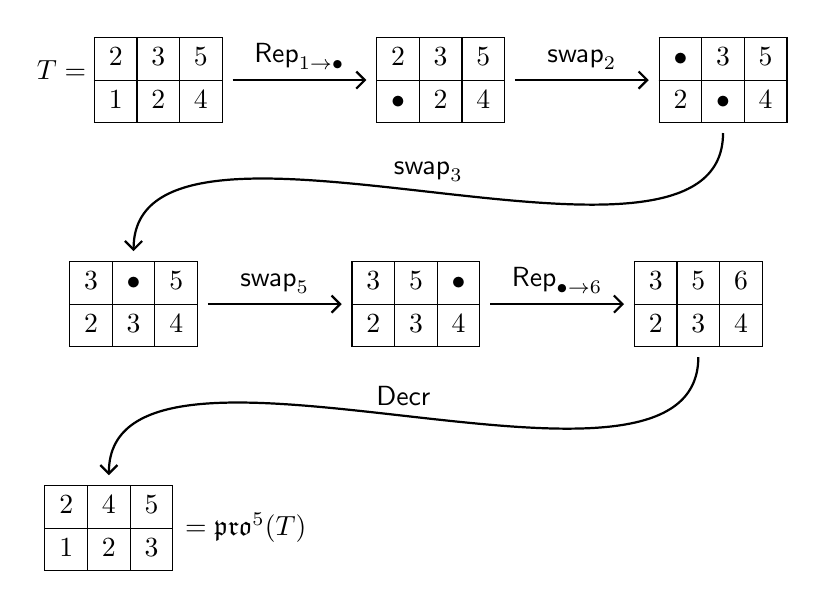
\begin{tikzpicture}
\node (T) {$T= \;$\ytableaushort{ 235,124}};
\node[right  = 1.7 of T] (T4) {\ytableaushort{ 235, \bullet 24}};
\node[right  = 1.7 of T4] (T5) {\ytableaushort{   \bullet 35, 2 \bullet 4}};
\node[below right  = 1.5 and -2.2 of T] (T6) {\ytableaushort{   3 \bullet 5, 234 }};
\node[right  = 1.7 of T6] (T7) {\ytableaushort{   35 \bullet, 234 }};
\node[right  = 1.7 of T7] (T9) {\ytableaushort{  356,234 }};
\node[below right = 1.5 and -2.2 of T6] (T10) {\ytableaushort{245,123}};
\node[right = -0.1 of T10] (pro) {$=\pro^{5}(T)$};
\path (T) edge[pil]  node[above]{$\rep_{1 \rightarrow \bullet}$} (T4);
\path (T4) edge[pil] node[above]{$\swap_2$} (T5);
\draw[->, thick] (T5.south) .. node[above]{$\swap_3$} controls ([yshift=-3cm] T5) and ([yshift=3cm] T6) .. (T6.north);
\draw[->, thick] (T9.south) .. node[above]{$\decr$} controls ([yshift=-3cm] T9) and ([yshift=3cm] T10) .. (T10.north);
\path (T6) edge[pil] node[above]{$\swap_5$} (T7);
\path (T7) edge[pil] node[above]{$\rep_{\bullet \rightarrow 6}$} (T9);
\end{tikzpicture}
\caption{The calculation of the $K$-promotion $\pro^{5}(T)$ of the increasing tableau $T$ through the action of a sequence of swaps.}\label{fig:promotion_via_swaps}
 \end{figure}

Using this characterization of $\pro^q$, we give names to the intermediate products of this process.
For $T \in \inc^q(\lambda)$, we define the tableau $T^{(N)}: \lambda \rightarrow \lbrace 2, \dots, q, \bullet \rbrace$ by 
\[T^{(N)} \coloneqq \swap_N \circ \cdots \circ \swap_2 \circ \rep_{1 \rightarrow \bullet}(T)\] for $N > 1$ and $T^{(1)} \coloneqq \rep_{1 \rightarrow \bullet}(T)$. We define the associated order ideal 
\[
\lambda \left( T^{(N)} \right) \coloneqq \left( T^{(N)} \right)^{-1}(\{2,\dots,N\})
\]
 to be the set of boxes of $T^{(N)}$ containing entries from $\{2,\dots,N\}$. Finally, define 
 \[
 T_N \coloneqq T^{(N)} \vert_{\lambda \left( T^{(N)} \right) }.
 \]
  Intuitively, $T^{(N)}$ shows $T$ at the point in $K$-promotion at which the boxes labeled $2$ through $N$ have been acted upon by $\swap$ operators, while $T_N$ is the restriction of $T^{(N)}$ to this subset of boxes. Examples of these intermediate tableaux appear in Figure~\ref{fig:restricted_promotions}. 
  
  The following lemmas use these intermediate products to show that $K$-promotion acts on a gappy tableau in essentially the same way and as on its deflation, provided that the gappy tableau contains at least one $1$. The following simple, but important, result shows why this condition on content is necessary.

\begin{lemma}\label{lem:no_ones}
If $\compress^q(T)\lbrace 1 \rbrace = 0$, then $\pro^q(T) = \decr(T)$. 
\end{lemma} 
\begin{proof}
If $\compress^q(T)\lbrace 1 \rbrace = 0$, then $\rep_{1 \rightarrow \bullet}(T) = T$. But then $\swap_\ell(T) = T$ for all $\ell$, since there are no nontrivial short ribbons containing the labels $\bullet$ and $\ell$. Also, $\rep_{\bullet \rightarrow 1}(T) = T$, since there is not $\bullet$ label in $T$. Therefore, $\decr$ is the only operator in Equation~(\ref{eq:kprodef2}) that acts nontrivially on $T$. 
\end{proof}

\begin{figure}[h]
%\includegraphics[scale=.35]{lemma_4p2.jpg}
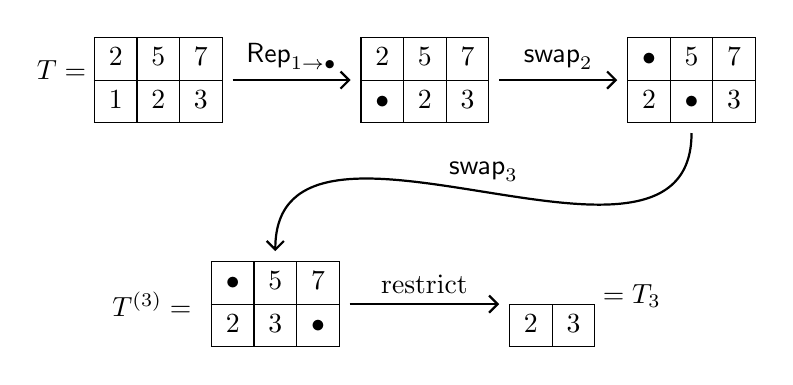
\begin{tikzpicture}
\node (T) {$T = \ytableaushort{257,123}$};
\node[right=1.5 of T] (D) {\ytableaushort{257,\bullet 23}};
\node[right = 1.5 of D] (T2) {\ytableaushort{\bullet 57,2 \bullet 3}};
\node[below right = 1.5 and -0.4 of T] (T3) {\ytableaushort{\bullet 5 7,23 \bullet}};
\node[left = 0 of T3] (mytag) {$T^{(3)}=$};
\node[right = 1.9 of T3] (Tres3) {\ytableaushort{\none,23} $\; = T_3$};
%\node[above left = -.2 and -0.7 of D] (fake1) {};
%\node[above left = -.2 and -2.0 of D] (fake2) {};
\path (T) edge[pil] node[above]{$\rep_{1 \rightarrow \bullet}$} (D);
\path (D) edge[pil] node[above]{$\swap_2$} (T2); 
\path (T3) edge[pil] node[above]{restrict} (Tres3);
\draw[->, thick] (T2.south) .. node[above]{$\swap_3$} controls ([yshift=-3cm] T2) and ([yshift=3cm] T3) .. (T3.north);
%\path (fake2) edge[pil, out=90, in=90, looseness=1.5] node[above]{$\swap_1$} (fake1);
\end{tikzpicture}
\caption{The tableau $T^{(3)}$ is obtained from $T$ by applying in sequence the operations 
$\rep_{1 \rightarrow \bullet}$, $\swap_2$, and $\swap_3$. 
We then obtain $T_3$ from $T^{(3)}$ by restricting to 
those boxes with labels less than or equal to $3$. The order ideal
 $\lambda \left( T^{(3)} \right)$ is the 
shape of the tableau $T_3$. }\label{fig:restricted_promotions}
\end{figure}

%-- not obvious that $\lambda$  is a shape but don't think need this here -- 
\begin{lemma} \label{lem:bullet_placement}
Let $T \in \inc^q(\lambda)$ with $\content^q(T) \lbrace 1 \rbrace = 1$. Let $i_k = \inflate^q_{\content^q(T)}(k)$ for $k = 1,...,N_T$. Then, for all $\x \in \lambda$ and $1 \leq k \leq N_T$, we have
 \begin{equation}\label{eq:gappy_promotion2}
\deflate^q(T)^{(k)}(\x) = \bullet \text{ if and only if } T^{(i_k)}(\x) = \bullet.
\end{equation}
\end{lemma}
\begin{proof} We proceed by induction on $k$. Fix $T \in \inc^q(\lambda)$  with $\content^q(T) \lbrace 1 \rbrace = 1$. In the base case $k = 1$,  $T^{(i_1)} = T^{(1)} = \rep_{1 \rightarrow \bullet}(T)$ has $\bullet$ in exactly those boxes $\x \in \lambda$ such that $T(\x) = 1$. On the other hand, $\deflate^q(T)^{(1)} =  \rep_{1 \rightarrow \bullet}(\deflate^q(T))$ has $\bullet$ in exactly those boxes $\x \in \lambda$ such that $\deflate^q(T)(\x) = 1$. But since $\content^q(T) \lbrace 1 \rbrace = 1$, $\deflate^q(T)(\x) = 1$ if and only if $T(\x) = 1$. 


Now, say the lemma holds for all tableaux $T$ in the case $k < t$. First consider the case where $T^{(i_t)}(\x) = \bullet$ and $T^{(i_{t-1})}(\x) \neq \bullet$. This is equivalent to the statement that $T^{(i_{t-1})}(\x) = i_t$ and $T^{(i_{t-1})}(\x') = \bullet$ for some $\x'$ adjacent to $\x$. But since $\rep_{1 \rightarrow \bullet}$ and $\swap_j$ for  $j \leq i_{t-1}$ only act on elements of $T$ labeled with $\bullet$'s or values less than or equal to $i_{t-1}$, $T^{(i_{t-1})}(\x) = i_t$ implies that $T^{(i_{t-1})}(\x) = T(\x) = i_t$. This is, in turn, equivalent by Theorem~\ref{thm:compressbijective} to the statement $\deflate^q(T)(\x) = t$, implying that $\deflate^q(T)^{(t-1)}(\x) = t$. Additionally, by the inductive hypothesis, $T^{(i_{t-1})}(\x') = \bullet$ if and only if $\deflate^q(T)^{(t-1)}(\x') = \bullet$. Therefore, the conditions of this case are equivalent to the conditions $\deflate^q(T)^{(t)}(\x) = \bullet$ and $\deflate^q(T)^{(t-1)}(\x) \neq \bullet$, as desired. 

Consider the other possible case, where $T^{(i_t)}(\x) = \bullet$ and $T^{(i_{t-1})}(\x) = \bullet$. This scenario is equivalent to the statement that $T^{(i_{t-1})}(\x) = \bullet$ and there is no $\x'$ adjacent to $\x$ such that $T^{(i_{t-1})}(\x') = i_t$. By similar reasoning as in the previous case, the second condition is equivalent to the statement that there is no $\x'$ adjacent to $\x$ with $T(\x') = i_t$. This statement is, in turn, equivalent to saying that there is no $\x'$ adjacent to $\x$ with $\deflate^q(T)(\x') = \deflate^q(T)^{(t-1)}(\x') = t$. Since $\deflate^q(T)^{(t-1)}(\x) = \bullet$ by the inductive hypothesis, the conditions of this case are finally equivalent to the conditions that $\deflate^q(T)^{(t)}(\x) = \bullet$ and $\deflate^q(T)^{(t-1)}(\x) = \bullet$, and we are done.
\end{proof}

\begin{lemma} \label{lem:gappy_promotion}
Take $T$ and $i_1,...,i_{N_T}$ as in Lemma~\ref{lem:bullet_placement}. Then for $1 \leq k \leq N_T$, 
\begin{equation}\label{eq:gappy_promotion}
 \tinflate^q \Big( \deflate^q(T)_k, \content^q(T) \Big) = T_{i_k}. 
\end{equation}
That is, the two sides are identical functions on the same domain. 
\end{lemma}

\begin{proof}  We proceed again by induction on $k$. The base case $k=1$ is trivial, since if $T \in \inc^q(\lambda)$ is any tableau, then $\lambda \left( \deflate^q(T)^{(1)} \right)$ and $\lambda \left( T^{(1)} \right)$ are both the empty order ideal.
%To establish the base case for this $T$, note that all numerical entries of $\rep_{1 \rightarrow \bullet}(T)_{1}$ are at least $2$. Therefore, $\swap_1$ acts trivially, $\lambda(T^{(1)}) = \emptyset$, and $T_1 = T_{i_1}$ is the empty tableau. The same reasoning shows that $\lambda(\deflate^q(T)^{(1)})$ is the empty tableau. %

Now, assume that the lemma holds for all increasing tableaux $T$ in the case $k < t$. We first analyze the left side of Equation~(\ref{eq:gappy_promotion}). Take $\x \in \lambda\left( \deflate^q(T)^{(t)} \right)$. If $\x \in \lambda\left( \deflate^q(T)^{(t-1)} \right)$, then 
$[\deflate^q(T)^{(t-1)}](\x) \leq t-1$ and hence
\[
\left[ \swap_{t}(\deflate^q(T)^{(t-1)})\right](\x) = \deflate^q(T)^{(t-1)}(\x).
\]
 If instead
 \[\x \in \lambda\left(\deflate^q(T)^{(t)}\right) \setminus \lambda\left(\deflate^q(T)^{(t-1)}\right),\]
  then either $[\deflate^q(T)^{(t-1)}](\x) = \bullet$ or $[\deflate^q(T)^{(t-1)}](\x) = t$. In the former case, there must be a box $\x'$ adjacent to $\x$ such that $[\deflate^q(T)^{(t-1)}](\x') = t$. In the latter case, we must have that for all boxes $\x'$ adjacent to $\x$, $[\deflate^q(T)^{(t-1)}](\x') \neq \bullet$. 

Now, we analyze the right side of Equation~(\ref{eq:gappy_promotion}). Take $\x \in \lambda\left( T^{(i_t)} \right)$.   If $\x \in \lambda \left(T^{(i_{t-1})} \right)$, then $\x \in \lambda(\deflate^q(T)^{(t-1)}) \subseteq \lambda(\deflate^q(T)^{(t)})$ by the inductive hypothesis. Further, this implies that $T^{(i_{t-1})}(\x) \leq i_{t-1}$,  and so we have
\[
\left[ \swap_{\ell+1} \left(T^{(\ell)} \right) \right](\x) = T^{(\ell)}(\x)
\]
 for all $i_{t-1} \leq \ell$. Therefore by the previous paragraph and the inductive hypothesis,
 \[ T^{(i_t)}(\x) = T^{(i_{t-1})}(\x) = \inflate^q_{\content^q(T)} \circ \deflate^q(T)^{(t-1)}(\x) =  \inflate^q_{\content^q(T)} \circ \deflate^q(T)^{(t)}(\x). \] This shows that Equation~(\ref{eq:gappy_promotion}) holds at $\x$. If $\x \in \lambda \left(T^{(i_{t})} \right) \setminus \lambda \left(T^{(i_{t-1})} \right)$, then $i_{t-1} < T^{(i_{t})}(\x) \leq i_t$. Thus, we must have that $T^{(i_{t})}(\x) = i_{t}$, since the $\swap$ operators do not change the content of a tableau. Therefore, either $T^{(i_{t-1})}(\x) = \bullet$ or $T^{(i_{t-1})}(\x) =  T(\x) = i_{t}$. In the former case, there must be a box $\x'$ adjacent to $\x$ such that $T^{(i_{t-1})}(\x') = T(\x') = i_{t}$. This occurs exactly when $\deflate^q(T)^{(t-1)}(\x') = \deflate^q(T)(\x') = t$. In the latter case, there is no $\x'$ adjacent to $\x$ such that $T^{(i_{t-1})}(\x') = \bullet$. Since we have assumed that  $\content^q(T) \lbrace 1 \rbrace = 1$, Lemma~\ref{lem:bullet_placement} implies that this occurs exactly when  $\deflate^q(T)^{(t-1)}(\x') \neq \bullet$ for every box $\x'$ adjacent to $\x$. Therefore each of these conditions is equivalent to the corresponding condition from the previous paragraph. 
 
Putting these facts together, we have shown that $\lambda \left(T^{(i_k)} \right) = \lambda \left(\deflate^q(T)^{(k)} \right)$ for all $k$, and that moreover, if $\deflate^q(T)_{k}(\x) = h$, then $T_k(\x) = \inflate^q_{\content^q(T)}(h)$. 
\end{proof}

\begin{remark}
As a corollary to Lemma~\ref{lem:gappy_promotion}, one can show that each $T_k$ is, in fact, in $\inc^q \left(\lambda \left( T^{(k)} \right) \right)$. However, we do not need this observation here.
\end{remark}

\begin{lemma}\label{lem:deflation_commutation}
Take $T$ and $i_1,...,i_{N_T}$ as in Lemma~\ref{lem:bullet_placement}. Then
\begin{equation}\label{eq:deflation_commutation}
\deflate^q \circ \pro^q(T) = \pro^{N_T} \circ \deflate^q(T).
\end{equation}

\end{lemma}
\begin{proof}
By Equation~(\ref{eq:kprodef2}), it is sufficient to show that
\begin{align*}
\deflate^q \circ &\decr \circ \rep_{\bullet \rightarrow q+1} \circ \swap_q \circ \cdots \circ \swap_1\circ \rep_{1 \rightarrow \bullet} (T) = \\
 & \decr \circ \rep_{\bullet \rightarrow N_T+1} \circ \swap_{N_T} \circ \cdots \circ \swap_1 \circ \rep_{1 \rightarrow \bullet} \circ \deflate^q (T). 
\end{align*}
Say $\x \not \in \lambda(T^{(q)})$; that is,  $T^{(q)}(\x) = \bullet$.  Then,
\[
[\decr \circ \rep_{\bullet \rightarrow q+1} \circ \swap_q \circ \cdots \circ \swap_1 (T)](\x) = q.
\]
Now by \cite[Lemma~2.1]{DPS}, the content vector of  
\[
\decr \circ \rep_{\bullet \rightarrow q+1} \circ \swap_q \circ \cdots \circ \swap_1 (T) = \pro^q(T)
\]
 is a cyclic rotation by one of the content vector of $T$. This implies that there are the same number of distinct labels in the content vector of $\pro^q(T)$, namely $N_T$, and, since $q$ is included, it must be the greatest such label, so 
 \[
 [\deflate^q \circ \decr \circ \rep_{\bullet \rightarrow q+1} \circ \swap_q \circ \cdots \circ \swap_1 (T)](\x) = N_T.
 \]
  On the other hand, since Lemma~\ref{lem:bullet_placement} implies that $\x \not \in \lambda(\deflate^q(T)^{(N_T)})$, we have
  \[
  [\decr \circ \rep_{\bullet \rightarrow N_T + 1} \circ \swap_{N_T} \circ \cdots \circ \swap_1 \circ \deflate(T)](\x) = N_T.
  \] 

Now say $\x \in \lambda(T^{(q)})$. We observe that since $\swap_\ell$ does not affect the tableau $\swap_{N_T} \circ \cdots \circ \swap_1 \circ \rep_{1 \rightarrow \bullet} (T)$ for $\ell > i_{N_T}$, we have that
\[ (\swap_q \circ \cdots \circ \swap_1 \circ \rep_{1 \rightarrow \bullet}( T ))_q = (\swap_{i_{N_T}} \circ \cdots \circ \swap_1 \circ \rep_{1 \rightarrow \bullet}( T ))_{i_{N_T}}.  \]
Therefore, it follows from Lemma~\ref{lem:gappy_promotion}, taking $k = N_T$, that 
\[ (\swap_q \circ \cdots \circ \swap_1 \circ \rep_{1 \rightarrow \bullet}( T ))_q = \inflate^q_{\content(T)} \circ (\swap_{N_T} \circ \cdots \circ  \rep_{1 \rightarrow \bullet} \circ \deflate^q(T)_{N_T}). \]

Now, since $\x \in \lambda(T^{(q)})$, we have that $T^{(q)}(\x) = \ell$ for $\ell \in \{2,3,\dots,q\}$. This implies that $\ell = i_k$ for some $2 \leq k \leq N_T$. Then, 
\[
\decr \circ \rep_{\bullet \to q+1} \circ \swap_q \circ \cdots \circ \swap_1 (T)(\x) = i_k-1.
\]
Because the content vector shifts cyclically, this implies that 
 \[
 [\deflate^q \circ \decr \circ \rep_{\bullet \rightarrow q+1} \circ \swap_q \circ \cdots \circ \swap_1 (T)](\x) = k-1.
 \]
  On the other hand, 
  \[
  [\swap_q \circ \cdots \circ \swap_1 \circ \deflate(T)](\x) = k,
  \]
   so 
   \[
   [ \pushQED{\qed} \decr \circ \rep_{\bullet \rightarrow N_T + 1} \circ \swap_{N_T} \circ \cdots \circ \swap_1 \circ  \deflate(T)](\x) = k-1. \qedhere \popQED \] \let\qed\relax
\end{proof}

\subsection{Computation of period}\label{sec:period} We use the results of the previous subsection to relate the period of $T \in \inc^q(\lambda)$ under $\pro^q$ to data concerning $\deflate^q(T)$. Let 
\[\Sigma^q: \lbrace 0,1\rbrace^q \rightarrow \lbrace 0,1\rbrace^q\]
 be the cyclic rotation defined by 
 \[
 \Sigma^q(v_1,...,v_q) = (v_2,...,v_q,v_1)
 \]
  for $(v_1,...,v_q) \in \lbrace 0,1 \rbrace^q$. 
  
\begin{theorem}\label{thm:periodthm}
Fix $T \in \inc^q(\lambda)$. Let $\tau$ be the the period of $\pro^{N_T}$ on $\deflate^q(T)$ and $\ell$ be the period of $\Sigma^q$ on $\content^q(T)$. If $d = q/\ell$, then the period of $\pro^q$ on $T$ is \[\frac{q/d \cdot \tau}{\mathrm{gcd}(N_T/d,\tau)}. \]
\end{theorem} 
    
  \begin{proof}
Define
  \[
  K^q: \coprod_{k \leq q}\incgl^k(\lambda) \times \binom{[q]}{k} \rightarrow \coprod_{k \leq q}\incgl^k(\lambda) \times \binom{[q]}{k}
  \] by
\[
K^q(S,v) =
\begin{cases}
    \big( \pro^{N_S}(S),\Sigma^q(v) \big),  & \text{if } v\{1\} = 1; \\        
   \big( S,\Sigma^q(v) \big), & \text{otherwise.}
\end{cases}
\]
We show that, for $T \in \inc^q(\lambda)$,
\begin{equation}\label{eq:k_commutes}
\compress^q \circ (\pro^q)^{\circ n}(T) = (K^q)^{\circ n} \circ \compress^q(T).
\end{equation}
Let \[ \pi_1: \coprod_{k \leq q}\incgl^k(\lambda) \times \binom{[q]}{k} \rightarrow \coprod_{k \leq q} \incgl^k(\lambda) \] be the projection onto the first factor and define $\pi_2$ similarly. It is immediate from the definitions that \[ \pi_2 \circ (K^q)^{\circ n} \circ \compress^q(T) = (\Sigma^q)^{\circ n} \circ \content^q(T)\] for all $n$. But by \cite[Lemma~2.1]{DPS},
\[  (\Sigma^q)^{\circ n} \circ \content^q(T) = \content^q \circ (\pro^q)^{\circ n} (T).\] This shows that the two sides of Equation~(\ref{eq:k_commutes}) are equal in the second factor.  

To show that Equation~(\ref{eq:k_commutes}) holds in the first factor, we proceed by induction on $n$. The base case $n = 0$ is tautological. Assume that Equation~(\ref{eq:k_commutes}) holds for $n-1$ and let \[ w \coloneqq \content^q \circ (\pro^q)^{\circ (n-1)}(T) = \pi_2 \circ (K^q)^{\circ (n-1)} \circ \compress^q(T). \]  By Theorem~\ref{thm:compressbijective}, we can write
\[ (\pro^q)^{\circ (n-1)}(T) = \inflate^q_{w} \circ (K^q)^{\circ (n-1)} \circ \compress^q(T).\] 
If $w\lbrace 1 \rbrace = 1 $, then
\begin{align*}
\pi_1 \circ \compress^q \circ (\pro^q)^{\circ (n)}(T) &= \deflate^q \circ (\pro^q)^{\circ (n)}(T) \\
&= \pro^{N_T} \circ \deflate^q \circ (\pro^q)^{\circ (n-1)}(T) &\text{Lemma~\ref{lem:deflation_commutation}, $w\lbrace 1 \rbrace = 1$} \\
&= \pro^{N_T} \circ \deflate^q \circ \inflate^q_{w} \circ (K^q)^{\circ (n-1)} \circ \compress^q(T)  \\
&= \pro^{N_T} \circ \pi_1 \circ (K^q)^{\circ (n-1)} \circ \compress^q(T) &\text{by Theorem~\ref{thm:compressbijective}} \\ 
&= \pi_1 \circ (K^q)^{\circ (n)} \circ \compress^q(T) &\text{because $w\lbrace 1 \rbrace = 1$.}
\end{align*}
On the other hand, if $w \lbrace 0 \rbrace = 0$, then 
\begin{align*}
\pi_1 \circ \compress^q \circ (\pro^q)^{\circ (n)}(T)) &= \deflate^q \circ (\pro^q)^{\circ (n)}(T) \\
&= \deflate^q \circ (\pro^q)^{\circ (n-1)}(T) &\text{by Lemma~\ref{lem:no_ones}, $w \lbrace 1 \rbrace = 0$} \\
&= \pi_1  \circ (K^q)^{\circ (n-1)} \circ \compress^q(T)  \\
&= \pi_1 \circ (K^q)^{\circ (n)} \circ \compress^q(T) &\text{because $w\lbrace 1 \rbrace = 0$.}
\end{align*}
This completes the proof of Equation~\ref{eq:k_commutes}.

Now, since $\compress^q$ is an injection, $(\pro^q)^{\circ n}(T) = T$ exactly when $\compress^q \circ (\pro^q)^{\circ n}(T) = \compress^q \circ T$. So we are reduced to looking at what powers $n$ of $K^q$ stabilize $\compress^q(T)$.
 

 
Say $n$ satisfies this property. Projecting onto the second factor, we must have that \[ (\Sigma^q)^{\circ n}(\content^q(T)) = \content^q(T), \] so $n = t \ell$ for some integer $t$, where $\ell$ is the period of $\content^q(T)$ under $\Sigma^q$.  Projecting onto the first factor, we must have that  \[ \pro^{n'}(\deflate^q(T)) = \deflate^q(T), \] where $n'$ is $n$ minus the number of times that $\content^q \circ (K^q)^{\circ j} \circ \compress(T) \lbrace 1 \rbrace = 0$ for $j \in \{ 0, \dots, n-1 \}$. If there are $r \cdot (q/\ell)$ zeros in $\content^q(T)$ and $n = t \ell$, then $n' = t \cdot(\ell - r)$. By our assumption on $n$, if $\tau$ is the order of $\pro^{N_T}$ on $\deflate^q(T)$, then $s \tau = n' = t(\ell - r)$ for some $s$.

Therefore, $(K^q)^{\circ n}  \circ \compress^q(T) = \compress^q(T)$ if and only if $n = t \ell = s \tau + t  r$ for positive integers $s$ and $t$. Hence, the order of $\pro^q$ on $T$ is equal to the least positive integer that can be simultaneously written in the forms $t \ell$ and $s \tau + t r$ for the same value of $t$. But $t \ell = s\tau + tr$ implies that $t(\ell-r) = s\tau$. Since $0 \leq r < \ell$, the least such $t \ell$ is clearly achieved when $t$ is minimal, which occurs when $t(\ell-r)$ is minimal, namely the least common multiple of $\ell-r$ and $\tau$. Thus, the least such $n$ can be expressed as 
\begin{equation}\label{eq:period}
n = t \ell = \frac{\ell \, \text{lcm}(\ell-r,\tau)}{\ell-r} = \frac{\ell \tau}{\text{gcd}(\ell-r,\tau)}.
\end{equation}
But if $d = q/\ell$, then $r = (q-N_T)/d$, so \[ \ell - r = q/d - (q-N_t)/d = N_T/d.\]
Therefore
\[ n = \frac{q/d \cdot \tau}{\text{gcd}(N_T/d,\tau)}, \]
as desired. 
\end{proof}

The following corollary will allow us to determine the period of $\pro$ in Section~\ref{sec:arithmetic}. 
\\
\begin{corollary}~\label{corr:pdbound}
In the notation of Theorem~\ref{thm:periodthm}, say that $\tau$ divides $k N_T$ for some $k \in \mathbb{N}$. Then the period of $\pro^q$ on $T$ divides $k q$. 
\end{corollary} 
\begin{proof}
First say $\tau = k N_T$. Then
\begin{equation}~\label{eq:pdbound} \frac{q/d \cdot \tau}{\text{gcd}(N_T/d,\tau)} = \frac{q/d \cdot k N_T}{\text{gcd}(N_T/d,k N_T)} = \frac{q/d \cdot k N_T}{N_T/d} = kq. 
\end{equation}
Now say $\tau = s \tau'$ for some $s \in \mathbb{N}$. For any integer $n$, $\tau'/\gcd(\tau',n)$ divides $s \tau'/\gcd(s \tau',n)$. Applying this fact to the leftmost term in Equation~\ref{eq:pdbound}, it follows that the period associated to $\tau'$ divides $k q$. 


\end{proof}
\section{The equivariant bijection}\label{sec:equivariant}

A more general approach to the ideas in this section was developed independently in \cite{Dilks.Striker.Vorland}. We give a complete development here, as the ideas are simpler in our more restrictive setting.

\subsection{Bijection between plane partitions and increasing tableaux.} 

Let $\{ \e_1, \e_2 \}$ be the standard basis for $\mathbb{Z}^{2}$ and let $\pi_i : \mathbb{Z}^{2} \to \mathbb{Z}$ be the projection map onto the $i$th coordinate. We say that a subset $\lambda \subset \mathbb{Z}^{2}$ is {\bf connected} if for all $\x,\x' \in \lambda$, there exist $r \in \mathbb{Z}_{\geq 0}$, $d_1,...,d_r \in \{1, 2 \}$, and signs $n_1,...,n_r \in \{ \pm 1 \}$ such that 
\[\left\{ \x + \sum_{k=1}^j n_k \e_{d_k} :  1\leq j \leq r \right\} \subseteq \lambda\]
 and $\x + \sum_{k=1}^r n_k \e_{d_k} = \x'$. Given these data, define $\x_0 = \x$ and $\x_\ell = \x + \sum_{k=1}^\ell n_k \e_{d_k}$ for $1 \leq \ell \leq r$. Then the sequence $\left( \x_\ell  \right)_{0 \leq \ell \leq r}$ is called a {\bf path of length} $r$. If $n_k = 1$ for all $k$, then the path is called a {\bf chain}. We call a finite nonempty connected subset of $\mathbb{Z}_{\geq 0}^2$ a {\bf shape}.  Shapes inherit a partial order from the natural componentwise partial order on $\mathbb{Z}^2$, and we will conflate a shape $\lambda$ with the poset thereby induced on it. Note that the restriction of this partial order to a chain in $\lambda$ is a chain poset, justifying our double use of terminology. A shape poset $\lambda$ is ranked by restricting the standard rank function $\text{rk}(x_1,x_2) = x_1 + x_2$ on $\mathbb{Z}^2$ to the subset $\lambda$. Each minuscule poset $P$ can be realized as a shape by considering its diagram from Figure~\ref{fig:min_poset_E} or~\ref{fig:min_poset} and then embedding the diagram in $\mathbb{Z}^2$ in the obvious way, so that the bottom-leftmost box sits at the origin of $\mathbb{Z}^2$ and the cover relations in $P$ correspond to cover relations in $\mathbb{Z}^2$. When we consider a minuscule poset $P$ as a shape, it will always be with respect to this particular embedding in $\mathbb{Z}^2$.

We say that the shape $\lambda$ is {\bf convex} if $\x\in \lambda$ and $\x + k  \e_d \in \lambda $ for some $d \in \{1, 2\}$ and $k \in \mathbb{Z}_{> 0}$ together imply  that $\{\x + j \e_d : 1 \leq j \leq k-1 \} \subseteq \lambda.$

For any shape $\lambda$, let \[a_i(\lambda) = \max \{ \pi_i(\x) \colon \x \in \lambda\}\] and \[\aaa_\lambda = \big(a_1(\lambda),a_{2}(\lambda)\big) \in \mathbb{Z}^2.\] We say the shape $\lambda$ is {\bf justified} if $(0,0) \in \lambda$ and $\aaa_{\lambda} \in \lambda$. Note that the minuscule posets are convex and justified, when considered as shapes as above. For any shape $\lambda$, define 
\[
\lambda^\star \coloneqq \lbrace \aaa_\lambda - \x: \x \in \lambda \rbrace.
\] It is clear that $\lambda^{\star}$ is a shape and that if $\lambda$ is convex (resp.\ justified), then $\lambda^\star$ is convex (resp.\ justified).  Define the {\bf rank} of $\lambda$ to be
\[ 
\rank(\lambda) \coloneqq \max_{\x \in \lambda} \rank(\x).
\]

The following elementary lemmas determine useful characteristics of the shapes considered in this paper. 

\begin{lemma} \label{lem:convex_chain}
Let $\lambda$ be a convex shape and let $\x,\x' \in \lambda$ be distinct. If $\x < \x'$, then $\lambda$ contains a chain from $\x$ to $\x'$. 
\end{lemma}

\begin{proof} 
Let $\x = (i,j)$ and $\x' = (i',j')$. Because $\x < \x'$, we have $i \leq i'$ and $j \leq j'$. Since $\lambda$ is a shape, there is at least one path from $\x$ to $\x'$. Take such a path $\mathscr{P} = (\x_{\ell})_{0\leq \ell \leq r}$ of minimal length, characterized by directions $d_1,...,d_r \in \{ 1,2 \}$ and signs $n_1,...,n_r \in \{ \pm 1\}$.  We claim that $\mathscr{P}$ is a chain. 

If not, then $n_t  = -1$ for some $1 \leq t \leq r$. Let $t$ be the least such index. For  $0 \leq \ell \leq r$, define $(i_\ell, j_\ell) = \x_\ell$, so that in particular $(i_0, j_0) = (i,j)$ and $(i_r, j_r) = (i',j')$.


Since $n_t = -1$, either $i_t = i_{t-1} -1$ or $j_t = j_{t-1} -1$.  Without loss of generality, we may assume $i_t = i_{t-1} -1$. 

Suppose there is no $h < t$ with $d_h = d_t$ and $n_h = 1$. Then $i_t = i_0 - 1$. Furthermore, since $i' = i_r \geq i_0$, there must be a least $k > t$ such that $i_k = i_0 = i_{t-1}$. Let $q = j_k - j_{t-1} $. Then clearly the subpath $(\x_{\ell})_{t-1\leq \ell \leq k}$ of $\mathscr{P}$ has length at least $|q| + 2$.
However by convexity, the path 
\[
\bigg( (i_{t-1}, j_{t-1}),   (i_{t-1}, j_{t-1} + \frac{q}{|q|}), (i_{t-1}, j_{t-1} + 2\frac{q}{|q|}), \dots , (i_{t-1}, j_{t-1} + |q|\frac{q}{|q|}) \bigg)
\]
of length $|q|$ from $(i_{t-1}, j_{t-1})$ to $(i_k, j_k)$ lies entirely inside $\lambda$, contradicting the minimality of $\mathscr{P}$.

Otherwise, consider the greatest $h < t$ with $d_h = d_t$ and $n_h = 1$. Then $i_{h-1} = i_t$. By minimality of $t$, we have $j_t \geq j_{h-1}$. Let $q = j_t - j_{h-1}$. Now the subpath $(\x_{\ell})_{h-1\leq \ell \leq t}$ of $\mathscr{P}$ has length $q + 2$. However by convexity, the path 
\[
\big( (i_{h-1}, j_{h-1}),   (i_{h-1}, j_{h-1} + 1), (i_{h-1}, j_{h-1} + 2), \dots , (i_{h-1}, j_{h-1} + q) \big)
\]
of length $q$ from $(i_{h-1}, j_{h-1})$ to $(i_t, j_t)$ lies entirely inside $\lambda$, contradicting the minimality of $\mathscr{P}$.
%If $i_t \geq i'$, then certainly $i_t \geq i = i_0$, so $t \geq 2$ and $i_t = i_{t-k}$ for some $k > 0$. If instead $i_t < i'$, then there must be some  $t < s \leq r$ with  $i_s = i_{t-1}$. Thus in both cases there are $u,v$ with $0 \leq u \leq r$ and $0 \leq v \leq r$ such that $i_u = i_v$ and $n_w  = -1$ for $u < w \leq v$. 
%But by convexity, all elements $(i_u,x)$ for $x \in (j_u,j_v)$ (or $(j_v,j_u)$) are contained in $\lambda$. Now the direct path along these elements has $\vert j_v-j_u \vert$ steps, while the path $(i_u,j_u),(i_{u+1},j_{u+1}),...,(i_v,j_v)$ must have at least $\vert j_v-j_u \vert + 2$ steps, since it has at least $\vert j_v - j_u \vert$ steps along the second dimension and at least two steps along the first dimension, one in the negative direction and one to cancel it out. This contradicts the minimality of this path, so no such $t$ exists and the path is a chain.  
\end{proof}

\begin{lemma}\label{lem:max_chain_same}
Let $\lambda$ be a convex justified shape. Then every maximal chain has length $a_1(\lambda) + a_2(\lambda)$. 
\end{lemma}
\begin{proof} 
Since for all $\x \in \lambda$ we have $(0,0) \leq \x$ and $\x \leq (a_1(\lambda),a_2(\lambda))$, all maximal chains must start at $(0,0)$ and end at $(a_1(\lambda),a_2(\lambda))$ by Lemma~\ref{lem:convex_chain}. But clearly any chain between these two elements has the desired length.
\end{proof} 

For a convex shape $\lambda$, an increasing tableau on the poset $\lambda$ is equivalent to a map $T: \lambda \rightarrow \mathbb{Z}_{>0}$ such that whenever $\x \in \lambda$ and $\x+\e_i \in \lambda$ for $i \in \lbrace 1,2 \rbrace$, then $T(\x) < T(\x+\e_i)$. The {\bf height} of an increasing tableau $T$ is the maximum value in its range. Recall that $\inc^q(\lambda)$ is the set of all increasing tableaux of height at most $q$ and base $\lambda$. 

Fix a convex justified shape $\lambda$ and $m \in \mathbb{Z}_{> 0}$. Now, we define a poset
\[
\lambda \times \mathbf{m} \coloneqq \{ (\x, y) \in \mathbb{Z}^3: \x \in \lambda, 0 \leq y \leq  m-1 \},
\] with the partial order given by restricting the natural partial order on $\mathbb{Z}^3$, that is
\[{\sf p} \geq {\sf q} \text{ if and only if } {\sf p}  - {\sf q} \in \mathbb{Z}_{\geq 0}^3.\] Note that, as a abstract poset, $\lambda \times \mathbf{m}$ is, in fact, isomorphic to the product of the posets $\lambda$ and $\mathbf{m}$; it is useful to us, however, to consider $\lambda \times \mathbf{m}$ as embedded inside $\mathbb{Z}^3$ in this particular fashion.


Recall that for any poset $P$, we write $J(P)$ for the collection of all order ideals of $P$.  
 Define the map $\Omega : J(\lambda \times \mathbf{m}) \rightarrow \inc^{\rank(\lambda)+ m+1}(\lambda^\star)$ as follows. 
% We write $2^A$ for the power set of a set $A$. 
 First, define the function 
 \[
 \mathrm{ht}: \mathbb{Z}_{\geq 0}^2 \times 2^{(\mathbb{Z}_{\geq 0}^3)} \rightarrow \mathbb{Z}_{\geq 0}
 \] (where $2^{(\mathbb{Z}_{\geq 0}^3)}$ denotes the power set of $\mathbb{Z}_{\geq 0}^3$) by 
 \[ \mathrm{ht}(\x,S) \coloneqq  \# \{ y \in \mathbb{Z}_{\geq 0} : (\x,y) \in S \}.  \]  
Intuitively, if an order ideal $I$ of $\lambda \times \mathbf{m}$ is viewed as a pile of blocks stacked on $\lambda \subset \mathbb{Z}^2$, then $\mathrm{ht}(\x,I)$ counts the number of blocks stacked in the column over $\x \in \lambda$. In this notation, $J(\lambda \times \mathbf{m})$ is exactly the set of all plane partitions with $\mathrm{ht}$ at most $m$ over the shape poset $\lambda$. Next, define $\Omega: J(\lambda \times \mathbf{m}) \rightarrow \inc^{\rank(\lambda) + m + 1}(\lambda^{\star})$ such that 
\[ [\Omega(I)]( \x )= \mathrm{ht}(\aaa_\lambda - \x,I) + \rank(\x)+1.\] 

\begin{proposition}\label{prop:bijection}
If $\lambda$ is a convex justified shape, then  $\Omega$ is a bijection.
\end{proposition}
\begin{proof}
Since $\lambda$ is justified and convex, $\lambda^\star$ has an element of rank $0$ and, by Lemma~\ref{lem:max_chain_same}, all maximal chains in $\lambda^\star$ have equal length. Hence the function $\Omega$ coincides with the map from \cite[Proposition~8.2]{HPPW}, and so by \cite[Proposition~8.2]{HPPW} we have that $\Omega$ is a bijection between plane partitions over $\lambda$ and increasing tableaux over $\lambda^\star$.
\end{proof}

Note, in particular, that Proposition~\ref{prop:bijection} applies to all of the minuscule posets, realized as convex justified shapes as in Figures~\ref{fig:min_poset_E} and~\ref{fig:min_poset}.

\subsection{Equivariance of $\Omega$.} 
In this section we prove Proposition~\ref{prop:equivariant}, our key to proving Theorems~\ref{thm:exceptionals} and~\ref{thm:propeller}. Proposition~\ref{prop:equivariant} is a mild extension of \cite[Lemma~4.2]{DPS} and our proof follows the same outline. We, however, still give significant details of the proof, as there are a few extra subtleties in our case.

The following gives an easy and useful way to determine whether a subset of $\lambda \times \mathbf{m}$ is an order ideal. 
\begin{lemma}\label{lem:whos_an_ideal?}
Let $\lambda$ be any shape. The subset $Q \subseteq \lambda \times \mathbf{m}$ is an order ideal if and only if both
\begin{itemize}
\item[(a)] $(i,j,k) \in Q$ implies that $(i,j,k') \in Q$, for $0 \leq k' \leq k$; and
\item[(b)] $(i,j) \geq (i',j')$ implies that $\mathrm{ht}((i,j),Q) \leq \mathrm{ht}((i',j'),Q)$.
\end{itemize}
\end{lemma}
\begin{proof} 
The ``only if'' direction is clear. 

Conversely, assume $Q$ satisfies $(a)$ and $(b)$. Consider $(i,j,k) \in Q$ and $(i',j',k') \in \lambda \times \mathbf{m}$ with $(i',j',k') \leq (i,j,k)$. We must show $(i',j',k') \in Q$. 

By assumption, $(i',j') \leq (i,j)$. Hence, by condition $(b)$, $\mathrm{ht}((i,j),Q) \leq \mathrm{ht}((i',j'),Q)$. Now, condition $(a)$ implies that, for all $\x \in \lambda$, we have \[ \mathrm{ht}(\x,Q) = 1 + \max \{ k'' \in \mathbb{Z}_{\geq 0} : (\x,k'') \in Q \}. \]  Applying this equality for $\x = (i,j)$ and $\x = (i'j')$, we conclude there is a $\hat{k} \geq k$ with $(i',j',\hat{k}) \in Q$. But since $k' \leq k \leq \hat{k}$, condition $(a)$ then implies $(i',j',k') \in Q$. 
\end{proof}

\begin{proposition}\label{prop:equivariant}
Let $\lambda$ be a convex justified shape. Then $\Omega$ intertwines $\mot_{\mathrm{id},(1,1,-1)}$ and $\pro^{\rank(\lambda)+m+1}$. That is, for $I \in J(\lambda \times \mathbf{m})$, we have \[
\Omega \circ \mot_{\mathrm{id},(1,1,-1)}(I) = \pro^{\rank(\lambda)+m+1} \circ \Omega(I).
\]
\end{proposition}
\begin{proof}
Let $a \coloneqq a_1(\lambda)$ and let $b \coloneqq a_2(\lambda)$; that is, let $(a,b) \coloneqq \aaa_{\lambda}$. Since $\lambda$ is justified, $a+b = \rank(\lambda)$.  Fix $I \in J(\lambda \times \mathbf{m})$. 

Recall that for $T \in \inc^{a+b+m+1}(\lambda)$, we have by definition that
\begin{equation*}
\pro^{a+b+m+1}(T) = \rho_{a+b+m} \circ  \cdots \circ \rho_1(T).
\end{equation*}
Since $-(m-1) \leq \langle (1,1,-1),(x,y,z) \rangle \leq a+b$ for $(x,y,z) \in \lambda \times \mathbf{m}$, we have
\begin{equation*}
\mot_{\mathrm{id},(1,1,-1)}(I) = \tau^{a+b-(a+b+m-1)}_{\mathrm{id},(1,1,-1)} \circ \cdots \circ \tau^{a+b}_{\mathrm{id},(1,1,-1)}(I).
\end{equation*}
Therefore, it suffices to show 
\begin{equation*}
\Omega \left(\tau^{a+b-(\ell-1)}_{\mathrm{id},(1,1,-1)}(I) \right) = \rho_\ell \left(\Omega(I)\right)
\end{equation*}
for all $\ell \in \{1, 2, \dots, a+b+m\}$. 

Fix such an index $\ell$ and a box $\y = (i,j) \in \lambda$. Let $Y \coloneqq I \cap ( \y \times \mathbf{m} )$ be the column of $\y$ in $I$. We consider the effect on $Y$ of applying $\tau^{a+b-(\ell-1)}_{\mathrm{id},(1,1,-1)}$ to the order ideal $I \in J(\lambda \times \mathbf{m})$ and the effect on the box $\aaa_\lambda - \y$ of applying $\rho_\ell$ to the increasing tableau $\Omega(I) \in \inc^{\rank(\lambda) + m + 1}(\lambda^{\star})$. Considering the definition of $\tau^{a+b-(\ell-1)}_{\mathrm{id},(1,1,-1)}$ from Equation~(\ref{eq:taudef}), note that $t_{(i,j,i+j-(a+b-(\ell-1))}$ is the unique toggle in that definition that acts on an element of $Y$.

Define the function $H : \lambda \to [m+1]$ by $H(\x) = \mathrm{ht}(\x,I)$ for $\x \in \lambda$.
By Lemma~\ref{lem:whos_an_ideal?}, observe that the function $H$ must be nonincreasing along any chain in $\lambda$. 
There are now four cases to consider depending on the value of $H(\y)$.

\medskip
\noindent
{\sf Case 1: $H(\y) > i+j-(a+b-(\ell-1))+1$:} 

Here, $(\y,i+j-(a+b-(\ell-1))) \in Y$, so $\tau^{a+b-(\ell-1)}_{\mathrm{id},(1,1,-1)}$ either removes this element from $Y$ or leaves $Y$ unchanged. Since, by the case assumption, $(\y,i+j-(a+b+(\ell-1))+1) \in Y$, removing $(\y,i+j-(a+b-(\ell-1)))$ from $I$ does not yield an order ideal. Therefore, the column $Y$ is unchanged by $\tau^{a+b-(\ell-1)}_{\mathrm{id},(1,1,-1)}$. On the other hand, the case assumption implies that $[\Omega(I)](\aaa_\lambda - \y) > \ell + 1$, so $\rho_{\ell}$ does not affect this entry of the increasing tableau $\Omega(I)$. 

\medskip
\noindent
{\sf Case 2: $H(\y) = i+j-(a+b-(\ell-1))+1$:} 

Here, $(\y,i+j-(a+b-(\ell-1))) \in Y$, while $(\y,i+j-(a+b-(\ell-1))+1) \notin Y$. We claim that $\tau^{a+b-(\ell-1)}_{\mathrm{id},(1,1,-1)}$ removes $(\y,i+j-(a+b-(\ell-1)))$ from $I$ exactly if $H(\y+\e_d) \leq i+j-(a+b-(\ell-1))$ for all $d \in \lbrace 1,2 \rbrace$ with $\y+\e_d \in \lambda$. 

For, on the one hand, if $\y+\e_d \in \lambda$ and $H(\y+\e_d) > i+j-(a+b-(\ell-1))$, then by Lemma~\ref{lem:whos_an_ideal?}, removing $(\y,i+j-(a+b-(\ell-1)))$ from $I$ would not leave an order ideal. 
On the other hand, say that $H(\y+\e_d) \leq i+j-(a+b-(\ell-1))$ for all such $d$. To verify that removing $(\y,i+j-(a+b-(\ell-1)))$ from $I$ results in an order ideal, consider any fixed $\y' = (i',j') \in \lambda$ with $\y' > \y$.  By Lemma~\ref{lem:whos_an_ideal?}, it is enough to check that 
$H(\y') \leq i+j-(a+b-(\ell-1)).$
Now, by Lemma~\ref{lem:convex_chain}, since $\y' > \y$, there is a chain from $\y$ to $\y'$. Clearly, this chain contains an element of the form $\y+\e_{d} \in \lambda$. But the function $H$ is nonincreasing along this chain, so $H(\y') \leq i+j-(a+b-(\ell-1))$, as desired.

On the tableaux side, the case assumption implies that $[\Omega(I)](\aaa_\lambda - \y) = \ell+1$. The $\aaa_\lambda - \y$ entry of $\Omega(I)$ is decreased to $\ell$ by $\rho_\ell$ exactly when, for all $d$ with $\aaa_\lambda - \y -\e_d \in \lambda^\star$, $[\Omega(I)](\aaa_\lambda - \y -\e_d) \leq \ell-1$. This is easily equivalent to the stated condition on when $\tau^{a+b-(\ell-1)}_{\mathrm{id},(1,1,-1)}$ acts nontrivially on $Y$.

\medskip
\noindent
{\sf Case 3: $H(\y) = i+j-(a+b-(\ell-1))$:}

Here, $(\y,i+j-(a+b-(\ell-1))-1) \in Y$ but $(\y,i+j-(a+b-(\ell-1))) \notin Y$. We claim that $\tau^{a+b-(\ell-1)}_{\mathrm{id},(1,1,-1)}$ adds $(\y,i+j-(a+b-(\ell-1)))$ to $I$ exactly when $H(\y-\e_d) \geq i+j-(a+b-(\ell-1))+1$ for all $d \in \lbrace 1,2 \rbrace$ with $\y-\e_d \in \lambda$. 

For, on the one hand, if $\y-\e_d \in \lambda$ and $H(\y-\e_d) < i+j-(a+b-(\ell-1))+1$, then by Lemma~\ref{lem:whos_an_ideal?}, adding $(\y,i+j-(a+b-(\ell-1)))$ to $I$ does not yield an order ideal. 
On the other hand, say that $H(\y-\e_d) \geq i+j-(a+b-(\ell-1))+1$ for all such $d$. To verify that adding $(\y,i+j-(a+b-(\ell-1)))$ to $I$ results in an order ideal, consider any fixed $\y' = (i',j') \in \lambda$ with $\y' < \y$. By Lemma~\ref{lem:whos_an_ideal?}, it is enough to check that $H(\y') \geq i+j-(a+b-(\ell-1))+1$. 
Now, by Lemma~\ref{lem:convex_chain}, since $\y' < \y$, there is a chain from $\y'$ to $\y$. Clearly, this chain contains an element of the form $\y-\e_d \in \lambda$. But the function $H$ is nonincreasing along this chain, so $H(\y') \geq i+j-(a+b-(\ell-1))+1$ as desired.

On the tableaux side, this case assumption implies that $[\Omega(I)](\aaa_\lambda - \y) = \ell$. The $\aaa_\lambda - \y$ entry of $\Omega(I)$ is increased to $\ell+1$ by $\rho_\ell$ exactly when, for all $d$ with $\aaa_\lambda - \y +\e_d \in \lambda^\star$, $[\Omega(I)](\aaa_\lambda - \y + \e_d)) \geq \ell+2$. This is easily equivalent to the stated condition on when $\tau^{a+b-(\ell-1)}_{\mathrm{id},(1,1,-1)}$ acts nontrivially on $Y$.

\medskip
\noindent
{\sf Case 4: $H(\y) < i+j-(a+b-(\ell-1))$:} 

Here, $(\y,i+j-(a+b-(\ell-1))) \notin Y$, so $\tau^{a+b-(\ell-1)}_{\mathrm{id},(1,1,-1)}$ either adds this element to $Y$ or else leaves $Y$ unchanged. Since, by the case assumption, $(\y,i+j-(a+b+(\ell-1))-1) \notin I$, by Lemma~\ref{lem:whos_an_ideal?}, adding $(\y,i+j-(a+b-(\ell-1)))$ to $I$ does not yield an order ideal. Therefore, the column $Y$ is unchanged by $\tau^{a+b-(\ell-1)}_{\mathrm{id},(1,1,-1)}$. On the other hand, the case assumption implies that $[\Omega(I)](\aaa_\lambda - \y) < \ell$, so $\rho_\ell$ does not affect this entry of $\Omega(I)$. 

\medskip
This completes the proof of Proposition~\ref{prop:equivariant}
\end{proof}

\begin{corollary}\label{cor:multisets}
Let $\lambda$ be a convex justified shape.
Then the multiset of cardinalities of $\Psi$-orbits on $J(\lambda \times \mathbf{m})$ and the multiset of cardinalities of $\pro^{\rank(\lambda)+ m+1}$-orbits on $\inc^{\rank(\lambda)+ m+1}(\lambda^\star)$ are equal.
\end{corollary}
\begin{proof}
By Proposition~\ref{prop:bijection}, $\Omega$ is a bijection between $J(\lambda \times \mathbf{m})$ and $\inc^{\rank(\lambda)+ m+1}(\lambda^\star)$. By Proposition~\ref{prop:equivariant}, the orbit structure of $\pro^{\rank(\lambda)+ m+1}$ on $\inc^{\rank(\lambda)+ m+1}(\lambda^\star)$ is the same as the orbit structure of $\mot_{\mathrm{id},(1,1,-1)}$ on $J(\lambda \times \mathbf{m})$. By Proposition~\ref{prop:psi_is_toggle}, the action of $\Psi$ on $J(\lambda \times \mathbf{m})$ is the same as the action of $\mot_{\mathrm{id},(1,1,1)}$. By Proposition~\ref{prop:conjugate_actions}, $\mot_{\mathrm{id},(1,1,1)}$ and $\mot_{\mathrm{id},(1,1,-1)}$ induce the same multiset of orbit cardinalities on $J(\lambda \times \mathbf{m})$.
\end{proof}

\section{Proof of Theorems~\ref{thm:exceptionals} and~\ref{thm:propeller}}\label{sec:arithmetic}
%
%Let $\binom{[q]}{k}$ be the collection of binary vectors of length $q$ with $k$ ones.  In the previous section, we defined the map 
%\[ \deflate\content: \inc^q(\lambda) \rightarrow \coprod_{1 \leq k \leq q} \incgl^k(\lambda) \times \binom{[s]}{r} \]
%for fixed $q$. We now write $\deflate\content^q$ (and $\deflate^q$, $\content^q$) for this fixed choice of $q$. We also define \[ F^r: \coprod_{s \in \mathbb{Z}_{>0}} V_{r,s} \rightarrow \mathbb{Z}^r \]
%where if $v$ has $r$ nonzero elements, then  $F(v) = F_v \in \mathbb{Z}^r$ is the map
%\[  k \mapsto \min_{n \in [1,...,N]} \bigg( \sum_{\ell = 1}^n v(\ell) = k \bigg). \]

%We saw in Section~\ref{sec:Kpro_defs} that $\compress^q : \inc^q(\lambda) \to \coprod_{0 \leq k \leq q} \incgl^k(\lambda) \times \binom{[q]}{k}$ is injective. Conversely, every $(T,v) \in \incgl^k(\lambda) \times \binom{[q]}{k}$ gives an element of $\inc^q(\lambda)$ in the following sense. Define the {\bf tableau inflation} map  \[ \tinflate^q: \coprod_{1 \leq k \leq q}  \incgl^k(\lambda) \times  \binom{[q]}{k}  \rightarrow  \inc^q(\lambda) \] such that if $(T,v) \in \incgl^k(\lambda) \times \binom{[q]}{k}$ then
%\[ \tinflate^q(T,v) \coloneqq \inflate^q_v \circ T \in \inc^q(\lambda)  \]  
%Note that
%\[ \compress^q \circ \tinflate^q(T,v) = (T,v). \] In particular, $\tinflate^q$ is injective. ! It is also surjective, since the image of $\compress^q$ is contained in the domain of $\tinflate^q$ and we showed in the previous section that for $T \in \inc^q(\lambda)$, $\tinflate^q \circ \compress^q(T) = T$. %
In this final section, we collect the above results into proofs of Theorems~\ref{thm:exceptionals} and~\ref{thm:propeller}. The remaining ingredients that we need to add are essentially calculations. Consider a poset $P$ that is either the Cayley-Moufang poset, the Freudenthal poset, or one of the propellers, and realize $P$ as a convex justified shape $\lambda$. By Corollary~\ref{cor:multisets},  the multiset of $\Psi$-orbit cardinalities for $J(\lambda \times \mathbf{m})$ equals the multiset of $\pro^{\rank(\lambda)+ m+1}$-orbit cardinalities for $\inc^{ \rank(\lambda)+ m+1}(\lambda^\star)$. Therefore, we may prove Theorems~\ref{thm:exceptionals} and~\ref{thm:propeller} by studying increasing tableaux instead of plane partitions. Denote the Cayley-Moufang shape by $\lambda_{CM}$, the Freudenthal shape by $\lambda_F$, and the propeller shape with $2k$ boxes ($k \geq 3$) by $\lambda_{k}$. Note that for each of these shapes $\lambda$, we have $\lambda = \lambda^\star$.

By Theorem~\ref{thm:compressbijective}, the $\pro$-orbit structure of increasing tableaux is controlled by the data of gapless increasing tableaux and binary vectors. But for any fixed $\lambda$, $\incgl(\lambda)$ is a finite set. Using a computer, we found all $549$ gapless increasing tableaux of shape $\lambda_{CM}$, as well as all $624\, 493$ gapless increasing tableaux of shape $\lambda_F$. For each such tableau $T \in \incgl^q(\lambda_{CM})$ or $\incgl^q(\lambda_F)$, we then determined the size of its orbit under $\pro^q$ by direct calculation. These data are given in Table~\ref{tab:E6} for $\lambda_{CM}$ and in Table \ref{tab:E7} for $\lambda_F$. 

\begin{table}[h]
\begin{tabular}{|c|c|c|}
\hline
$q$ & orbit size & number of orbits\\
  \hline
  11 & 1 & 1\\
  \hline
  12 & 3 & 1\\ \cline{2-3}
   & 12 & 1 \\
   \hline
  13 & 13 & 6\\
  \hline
  14 & 7 & 2\\\cline{2-3}
  & 14 & 12\\
  \hline
    15 & 15 & 13\\
  \hline
  16 & 2 & 1\\\cline{2-3}
   & 4 & 1\\\cline{2-3}
   & 8 & 1\\\cline{2-3}
  & 16 & 4\\
  \hline
\end{tabular}
\caption{The distribution of $\pro^q$-orbits of gapless increasing tableaux in $\incgl^q(\lambda_{CM})$ for each $q$.}
\label{tab:E6}
\end{table}

\begin{table}[h]
\begin{tabular}{|c|c|c|}
\hline
$q$ & orbit size & number of orbits\\
  \hline
  17 & 1 & 1\\
  \hline
  18 & 2 & 1\\ \cline{2-3}
   & 18 & 2 \\
   \hline
  19 & 19 & 30\\
  \hline
  20 & 20 & 228\\
  \hline
    21 & 7 & 3\\ \cline{2-3}
    & 21 & 1044 \\
  \hline
  22 & 22 & 3053\\\cline{2-3}
   & 66 & 2\\
  \hline
  23 & 23 & 5813\\ \cline{2-3}
  & 69 & 13 \\
   \hline
  24 & 8 & 7\\\cline{2-3}
   & 24 & 7195\\\cline{2-3}
   & 48 & 4\\\cline{2-3}
   & 72 & 26\\
   \hline
  25 & 25 & 5602\\ \cline{2-3}
  & 50 & 8 \\ \cline{2-3}
  & 75 & 21 \\
   \hline
  26 & 2 & 2\\ \cline{2-3}
  & 26 & 2495 \\ \cline{2-3}
  & 52 & 4 \\ \cline{2-3}
  & 78 & 6 \\
   \hline
 27 & 3 & 2\\ \cline{2-3}
  & 9 & 4 \\ \cline{2-3}
  & 27 & 484 \\
  \hline
\end{tabular}
\caption{The distribution of $\pro^q$-orbits of gapless increasing tableaux in $\incgl^q(\lambda_F)$ for each $q$.}
\label{tab:E7}
\end{table}

It is essentially trivial to observe that, for any $k$, $\incgl(\lambda_k)$ consists of exactly three increasing tableaux. There are two tableaux in $\incgl^{2k}(\lambda_k)$, forming a single $\pro^{2k}$-orbit, and a single tableau in $\incgl^{2k-1}(\lambda_k)$, which is necessarily fixed by $\pro^{2k-1}$. These three tableaux and their orbits are illustrated in Figure~\ref{fig:propeller_orbits} in the case $k=4$ (which is, in fact, completely generic). Table~\ref{tab:prop} records the observations of this paragraph in form analogous to Tables~\ref{tab:E6} and~\ref{tab:E7}.

\begin{figure}[h]
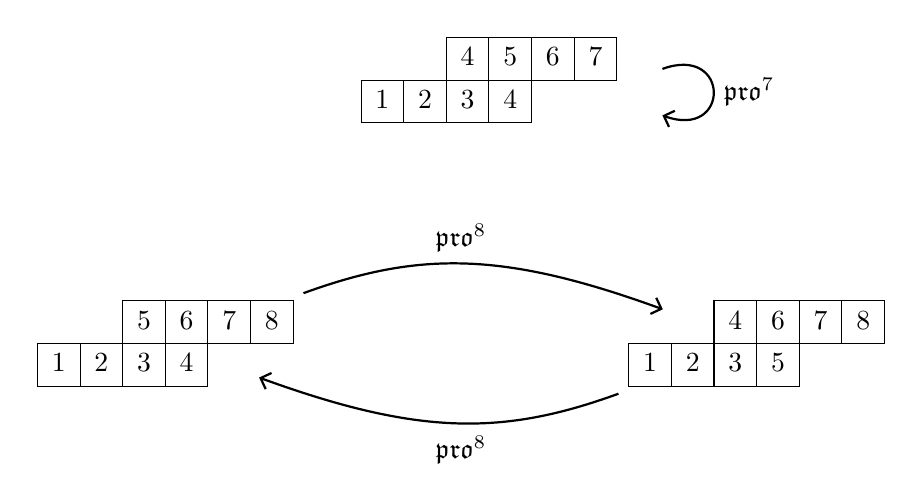
\begin{tikzpicture}
\node (T7) {\ytableaushort{\none \none 4567,1234}};
\node[above right = -0.7 and .2 of T7] (fake1) {};
\node[above right = -1.2 and .2 of T7] (fake2) {};
\node[below left = 2 and 0.6 of T7] (T8A) {\ytableaushort{\none \none 5678,1234}};
\node[right = 4 of T8A] (T8B) {\ytableaushort{\none \none 4678,1235}};
\path (T8A) edge[pil, out=20,in=160,shorten >=-6mm] node[above]{$\pro^8$} (T8B);
\path (T8B) edge[pil, out = 200, in=340,shorten >=-6mm] node[below]{$\pro^8$} (T8A);
\path (fake1) edge[pil, out = 20, in = 340, looseness=4] node[right]{$\pro^7$} (fake2);
\end{tikzpicture}
\caption{The set $\incgl(\lambda_4)$ consists of the three illustrated gapless increasing tableaux. The unique element of $\incgl^7(\lambda_4)$ forms a singleton $\pro^7$-orbit, while $\pro^8$ switches the two elements of $\incgl^8(\lambda_4)$, as shown. The situation for $k \neq 4$ is exactly analogous.}\label{fig:propeller_orbits}
\end{figure}

\begin{table}[h]
\begin{tabular}{|c|c|c|}
\hline
$q$ & orbit size & number of orbits\\
  \hline
  $2k-1$ & 1 & 1\\
  \hline
  $2k$ & 2 & 1\\ 
  \hline
\end{tabular}
\caption{The distribution of $\pro^q$-orbits of gapless increasing tableaux in $\incgl^q(\lambda_{k})$ for each $q$.}
\label{tab:prop}
\end{table}

 Additionally, we need the fact that the number of elements of $\binom{[M]}{k}$ of any fixed $\Sigma^M$-order is given explicitly by \cite[Theorem~1.1(b)]{Reiner.Stanton.White}:
\begin{theorem}[Reiner, Stanton, and White]\label{thm:rsw}
Let 
\begin{equation*}
f_{M,k}(q) \coloneqq 
\begin{cases}
 \frac{[M]!_q}{[k]!_q\cdot [M-k]!_q} & \text{if } M \geq k \\
 0 & \text{if } M < k 
\end{cases}
\end{equation*}
where $[\ell]!_q \coloneqq \prod_{i=1}^\ell [i]_q$ and $[i]_q \coloneqq \sum_{j = 0}^{i-1} q^j$ are the standard $q$-analogues. Then, 
\[\#\left\{ v \in \binom{[M]}{k} : (\Sigma^M)^{\circ s}(v) = v \right\} = f_{M,k}(\zeta^s),\] where $\zeta$ is any primitive $M$th root of unity. \qed
\end{theorem} 
We will use Theorems~\ref{thm:periodthm} and~\ref{thm:rsw}, together with the data of Tables~\ref{tab:E6},~\ref{tab:E7}, and~\ref{tab:prop}, to completely determine the multiset of $\pro^M$-orbit cardinalities on any set $\inc^M(\lambda)$ for $\lambda \in \{ \lambda_{CM}, \lambda_F, \lambda_k \}$. These tables, along with Corollary~\ref{corr:pdbound}, immediately give the period of $\pro^M$.
%NEED LOWER TOO

\begin{theorem}~\label{thm:actualpdbound}
For $M \gg 0$, the period of $\pro^M$ on $\inc^M(\lambda)$ is 
\begin{itemize}
\item $M$ for $\lambda = \lambda_k$, 
\item $M$ for $\lambda = \lambda_{CM}$, and 
\item $3M$ for $\lambda = \lambda_{F}$. 
\end{itemize}
(Here `$M \gg 0$' means $M \geq 2k$ for $\lambda = \lambda_k$, $M \geq 12$ for $\lambda = \lambda_{CM}$, and $M \geq 22$ for $\lambda = \lambda_{F}$.)
\end{theorem}
\begin{proof}
Inspecting Table~\ref{tab:E6} shows that, for $\lambda_{CM}$, the period of each gapless tableau (column 2) divides its height (column 1). By Corollary~\ref{corr:pdbound}, this implies that for any $M$, the $\pro^M$-period of each tableau divides $M$.
Whenever $M$ is at least $12$,  
it is always possible to find a tableau attaining period $M$ by taking a gapless tableau $T \in \incgl^{12}(\lambda_{CM})$ with period $12$ and then inflating according to a content vector with $\Sigma^M$-period $M$.

Similarly, inspecting Table~\ref{tab:E7} shows that, for $\lambda_F$, the period of all gapless tableaux of height $q$ divides $3q$ for each $q$. Therefore, Corollary~\ref{corr:pdbound} gives that for every $M$, the period of each tableau divides $3M$. Whenever $M$ is at least $22$, the period $3M$ is attained, since any gapless tableau  $T \in \incgl^{22}(\lambda_F)$ with period $66$ may be inflated according to a content vector of $\Sigma^M$-period $M$ to a height $M$ tableau of period $3M$. 

Finally, the analogous calculation for $\lambda = \lambda_k$ is easy by inspection of Table~\ref{tab:prop}.
\end{proof}

\begin{theorem}\label{thm:F_bad}
Conjecture~\ref{conj:rush.shi} holds for $\lambda_F$ only when $k \leq 4$.
\end{theorem}
\begin{proof}
That Conjecture~\ref{conj:rush.shi} holds for $\lambda_F$ in the case $k \leq 4$ is a straightforward calculation using Table~\ref{tab:E7}, Theorem~\ref{thm:periodthm}, and Theorem~\ref{thm:actualpdbound}. SHOULD SAY INSTEAD THAT IT'S MODELLED ON THE COMPUTATIONS BELOW, OR PROVE A VERSION FOR.  

It remains to show that the conjecture fails for $k \geq 5$. Hence, let $M \geq 22 = 5 +  \rank(\lambda_F) + 1$. By Theorem~\ref{thm:actualpdbound}, $\pro^{M}$ has order $3M$ on $\inc^{M}(\lambda_F)$. 

Suppose $T \in \inc^{M}(\lambda_F)$ were fixed by $\pro^{M}$.  By Equation~\ref{eq:period}, the $\Sigma^{M}$-period of $\content^{M}(T)$ is $1$. Since $\content^M(T)$ is certainly not a vector of all $0$'s, it must therefore be a vector of all $1$'s. Hence, $N_T = M$ and $\deflate(T) = T$. Therefore, $T$ is gapless. However, Table~\ref{tab:E7} shows that no element of $\incgl^{M}(\lambda_F)$ is fixed by $\pro^{M}$, for any $M \geq 22$, so such a $T$ does not exist.

%Therefore $\gcd{(N_T/d,\tau)} = 1$, where $\tau$ is the full-content period of the tableau. But then Equation~\ref{eq:period} implies that $\tau = 1$. However, there are no full-content tableau of height $22$ and orbit size $1$. Therefore, there are no tableau fixed by $\pro^{22}$. Theorem~\ref{thm:periodthm} and Table~\ref{tab:E7} allow us to compute that there are $0$ tableaux fixed by $\pro^{22}$.

Now let $\zeta$ be a primitive $(3M)$th root of unity. By the above, Conjecture~\ref{conj:rush.shi} claims that $f_{\lambda_F}(\zeta) = 0$. But this is impossible, for if $f_{\lambda_F}(\zeta) = 0$, then the cyclotomic polynomial $\Phi_{3M}$ would divide the numerator of $f_{\lambda_F}$, which is the product of polynomials of the form $1-x^m$ where $m < 3M$. Thus, Conjecture~\ref{conj:rush.shi} fails in these cases. 
\end{proof}

For specified $\lambda \in \{\lambda_k, \lambda_{CM}, \lambda_F\}$, we denote by $N_T\{i\}$, $\tau\{i\}$, and $N\{i\}$ the $i$th element of the first, second, and third columns of the corresponding table, respectively. 
\-\ \\ \-\

\begin{theorem}~\label{thm:mainresult}
Fix $\lambda \in \lbrace  \lambda_k, \lambda_{CM} \rbrace$, $M \gg 0$, and $d$ dividing $q$. Let $\mathcal{R}(\lambda,q,d)$ be the number of increasing tableaux $T \in \inc^q(\lambda)$ whose $\pro^q$-period divides $q/d$. Then,
\begin{equation}\label{eq:mainresulteq} 
\mathcal{R}(\lambda,q,d)  = \sum \limits_{i: \, d \, \vert \, \frac{N_T\{i\}}{\tau\{i\}}} \tau\{i\} \, N\{i\} \, f_{q,N_T}(\zeta^{q/d}).
\end{equation}
\end{theorem}
\begin{proof}
Theorem~\ref{thm:compressbijective} gives that tableaux of height $q$ correspond bijectively to pairs of gapless tableaux and content vectors of length $q$ with $N_T$ ones, where $N_T$ is the height of the gapless tableau. The table corresponding to $\lambda$ gives all possible gapless tableaux. We loop over the rows of the table and determine for each row how many content vectors yield height-$q$ tableaux whose periods divide $q/d$. 

For each $i$, let $\ell\{i\} = N_T\{i\}/\tau\{i\}$. Then $\ell\{i\}$ is an integer by Theorem~\ref{thm:actualpdbound}.  By Theorem~\ref{thm:periodthm}, a gapless tableau of height $N_T\{i\}$ and a content vector with period $q\{i\}/\tilde{d}$ give a tableau of period \[ \frac{\frac{q\{i\}}{\tilde{d}} \frac{N_T\{i\}}{\ell\{i\}}}{\gcd(\frac{N_T\{i\}}{\tilde{d}},\frac{N_T\{i\}}{\ell\{i\}})} = \frac{\frac{q\{i\}}{\tilde{d}} \frac{N_T\{i\}}{\ell\{i\}}}{\frac{N_T \, \gcd(\ell\{i\},\tilde{d})}{\tilde{d} \ell\{i\}}} = \frac{q\{i\}}{\gcd(\ell\{i\},\tilde{d})}. \] 
Therefore, the tableau has period dividing $q\{i\}/d$ is and only if $d$ divides both $\tilde{d}$ and $\ell\{i\}$. Now $d$ divides $\tilde{d}$ if and only if the period of the content vector divides $q\{i\}/d$. But the number of content vectors of length $q\{i\}$ with $N_T\{i\}$ ones and with period dividing $q\{i\}/d$ is precisely $f_{q,N_T}(\zeta^{q/d})$ (Theorem~\ref{thm:rsw}).
\end{proof}

In the cases $\lambda = \lambda_k$ and $\lambda = \lambda_{CM}$, the resulting formula is simple enough to check by hand. As in \cite[Proof of Theorem 7.1]{Reiner.Stanton.White}, we will need the following elementary identity, allowing us to work with integers rather than $q$-integers. 


\begin{lemma}\label{lem:evalq}
Let $\zeta$ be a primitive $N$th root of unity and let $d \divides N$. Then $[n]_{\zeta^{N/d}} = 0$ if and only if $n \equiv 0 \mod d$. Moreover, if $n_1 \equiv n_2 \mod d$, then 
\begin{equation}\label{eq:evalq}
\pushQED{\qed}
\lim \limits_{q \rightarrow \zeta^{N/d}} \frac{[n_1]_q}{[n_2]_q} = 
\begin{cases}
\frac{n_1}{n_2}, &\text{if }  n_1 \equiv n_2 \equiv 0 \mod d; \\
1, &\text{if } n_1 \equiv n_2 \neq 0 \mod d.
\end{cases} \qedhere \popQED
\end{equation}
\end{lemma}

For example, we evaluate $f_k(\zeta^{q/d})$ for some $d$ dividing both $q$ and $k$. By definition,
\[ f_k(\zeta^{q/d}) = \frac{[q-(2k-2)]_{\zeta^{q/d}}[q-(2k-2)+1]_{\zeta^{q/d}}...[q-(k-1)]_{\zeta^{q/d}}^2...[q-1]_{\zeta^{q/d}}[q]_{\zeta^{q/d}}}{[1]_{\zeta^{q/d}}[2]_{\zeta^{q/d}}...[k]_{\zeta^{q/d}}^2...[2k-2]_{\zeta^{q/d}}[2k-1]_{\zeta^{q/d}}}.\]
Lemma~\ref{lem:evalq} allows us to convert this to a ratio of polynomials by matching equivalence classes modulo $d$ in the numerator and denominator. We see that each term in the numerator has a corresponding term in the denominator. All ratios evaluate to $1$ except those divisible by $d$. Collecting these, we have
\[ f_k(\zeta^{q/d}) = \frac{(q-(2k-d)) ...  (q)}{(d) ...  (2k-d) k} = \frac{2k}{k}  \binom{q/d}{2k/d} = 2 \binom{q/d}{2k/d}\]    
as desired. 

An important special case allows us to improve Theorem~\ref{thm:rsw}. We have that for any $M, k \in \mathbb{Z}_{> 0}$, if $\zeta$ is an $M$th root of unity and $d$ divides $\gcd(M,k)$, then
\begin{equation}~\label{eq:evalstraightshape}
f_{M,k}(\zeta^{M/d}) = \binom{M/d}{k/d} = \frac{(M-(k-d))(M-(k-2d)) ...  (M-d)(M)}{(d)  (2d)  ...  (k-d) (k)}. 
\end{equation}
This equation holds even when $k > M$ because in this case, one of the numerator terms will be $0$. 



\begin{proof}[Proof of Theorem~\ref{thm:propeller}] Fix positive integers $k$, $q$, and $d$ dividing $q$. We have that \[ f_k(\zeta) = \frac{[q]!_q [q-(k-1)]_q}{[2k-1]!_q [q-(2k-1)]!_q [k]_q }.\]  If $d = 1$, then by Theorem~\ref{thm:mainresult}, 
\[ \mathcal{R}(\lambda_k,q,d) = f_{q,2k-1}(1) + 2 \, f_{q,2k}(1) = \binom{q}{2k-1} + 2 \binom{q}{2k} = \frac{(2q-2k+1)q!}{(2k)!(q-2k+1)!} = f_k(1). \]
Now for $d > 1$, we can have that $d$ divides $k$, or $d$ divides $2k-1$, or $d$ divides neither. If $d$ divides $k$, then by Equation~\ref{eq:evalstraightshape},
\[ \mathcal{R}(\lambda_k,q,d) = 2 \, f_{q,2k}(\zeta^{q/d}) = 2\binom{q/d}{2k/d} = f_k(\zeta^{q/d}).\]

If $d$ divides $2k-1$,  then
\[ \mathcal{R}(\lambda_k,q,d) =  f_{q,2k-1}(\zeta^{q/d}) = \binom{q/d}{(2k-1)/d} = f_k(\zeta^{q/d}).\]
If $d$ does not divide either $k$ or $2k-1$, then on the one hand Theorem~\ref{thm:mainresult} predicts that $\mathcal{R}(\lambda_k,q,d) = 0$, and on the other hand $d$ divides $\lceil{\frac{2k}{d}}\rceil$ of the terms in the numerator of $f_k(\zeta^{q/d})$ and $\lfloor{\frac{2k}{d}}\rfloor$ of the terms in the denominator, so $f_k(\zeta^{q/d}) = 0$. 
\end{proof}

The verification for $\lambda = \lambda_{CM}$ is equally straightforward. 

\begin{proof}[Proof of Theorem~\ref{thm:exceptionals}]
Theorem~\ref{thm:F_bad} proves the $\lambda_F$ cases. Hence, it remains to consider $\lambda = \lambda_{CM}$.

Inspecting Table~\ref{tab:E6}, we see that the possible values of $\ell\{i\} = N_T\{i\}/\tau\{i\}$ are $1,11,2,4$ and $8$. Therefore we evaluate $\mathcal{R}(\lambda_{CM},q,d)$ for each $d$ that divides one or more of these $\ell$ values. We verify that this matches the prediction given by $f^q_{CM}$, and that $f^q_{CM}$ predicts $\mathcal{R}(\lambda_{CM},q,d) = 0$ for all $d$ not dividing any of these integers.
\begin{itemize}
\item If $d$ divides $1$, then Theorem~\ref{thm:mainresult} predicts 
\begin{align*}
\mathcal{R}(\lambda_{CM},q,1) &= 1 \cdot 1 \cdot \binom{q}{11} + (3 \cdot 1  + 12 \cdot 1)  \cdot \binom{q}{12} + 13 \cdot 6 \cdot \binom{q}{13} + (7\cdot 2 + 14 \cdot 12) \binom{q}{14}  \\ &\ \ \ \ \ \ + 15 \cdot 13 \cdot \binom{q}{15} + (2 \cdot 1 + 4 \cdot 1 + 8 \cdot 1 + 16 \cdot 4) \binom{q}{16} \\
&= \frac{(q-10)(q-9)(q-8)(q-7)^2(q-6)^2(q-5)^2(q-4)^2(q-3)^2(q-2)(q-1)q}{1\cdot 2\cdot 3\cdot 4^2 \cdot 5^2 \cdot 6^2 \cdot 7^2 \cdot 8^2 \cdot 9 \cdot 10 \cdot 11} \\
&= f_{CM}^q(1).
\end{align*}
\item If $d$ divides $11$ but not $1$, Theorem~\ref{thm:mainresult} predicts
\begin{align*}
\mathcal{R}(\lambda_{CM},q,11) &= 1 \cdot 1 \cdot \binom{q/11}{11/11} \\
&= q/11 \\ 
&= f_{CM}^q(\zeta^{N/11}).
\end{align*}
\item If $d$ divides $8$ but not $4$, Theorem~\ref{thm:mainresult} predicts
\begin{align*}
\mathcal{R}(\lambda_{CM},q,8) &= 2 \cdot 1 \cdot \binom{q/8}{16/8} \\
&= \frac{(q)(q-8)}{8^2} \\
&= f_{CM}^q(\zeta^{N/8}).
\end{align*}
\item If $d$ divides $4$ but not $2$, Theorem~\ref{thm:mainresult} predicts
\begin{align*}
\mathcal{R}(\lambda_{CM},q,4) &= 3 \cdot 1 \cdot \binom{q/4}{12/4} + (4 \cdot 1 + 2 \cdot 1) \cdot \binom{q/4}{16/4}  \\
&= \frac{(q-8)(q-4)^2q}{4^2 \cdot 8^2} \\
&= f_{CM}^q(\zeta^{N/4}).
\end{align*}
\item If $d$ divides $2$ but not $4$, Theorem~\ref{thm:mainresult} predicts
\begin{align*}
\mathcal{R}(\lambda_{CM},q,2) &= 3 \cdot 1 \cdot \binom{q/2}{12/2} + 7 \cdot 2 \cdot \binom{q/2}{14/2} + (2 \cdot 1 + 4 \cdot 1 + 8 \cdot 1) \cdot \binom{q/2}{16/2} \\
&= \frac{(q-10)(q-8)(q-6)^2(q-4)^2(q-2)q}{10 \cdot 8^2 \cdot 6^2 \cdot  4^2 \cdot 2}\\
&= f_{CM}^q(\zeta^{N/2}).
\end{align*}
\end{itemize}
This exhausts all possible $d$ dividing one of the above integers. To see that the cyclic sieving polynomial predicts all other $d$ values are $0$, we first observe that $f_{CM}^q(\zeta^{N/d}) = 0$ if $d > 11$. For in this case, Lemma~\ref{lem:evalq} implies that one of the numerator terms (namely, $[q]_{\zeta^{N/d}}$) is zero, while none of the denominator terms are. 

Using the same identity to count zeros in the numerator and denominator, it is easily checked that the remaining values of $d \leq 11$ evaluate to $0$. 
\end{proof}

%We will also need the following elementary algorithm. We say that a quantity $F$ {\bf has the same dependence on $x$ and $x'$} if $F(x) = P(x)$ and $F(x') = P(x')$ for some polynomial $P$. A vector $(F^1,...,F^n)$ has the same dependence on $x$ and $x'$ if $F^i$ has the same dependence on $x$ and $x'$ for each $i$. 
%
%%That is, we must show that the number of tableaux fixed by $\pro^d$ is equal to $f_{\lambda}^m(\zeta^d)$ for $\zeta$ an $M$th root of unity. Now
%%Fix a shape $\lambda$ with maximum rank $r$ and $s$ boxes.  A gapless tableau on $\lambda$ must have its maximum label between $r+1$ and $s$.  Theorem~\ref{thm:compressbijective} shows that each tableaux of height $q$ corresponds uniquely to an element of $\incgl^k(\lambda) \times \binom{[q]}{k}$ for some $k \leq q$. Further, each element of $\binom{[q]}{k}$ has a period (under cyclic permutation) which is a divisor of $q$. ! Therefore to determine the number of tableaux $S \in \inc^q(\lambda)$ whose period divides a given positive integer $L$, we can execute the following algorithm.
%
%\begin{algorithm}\label{alg:2}
%\hspace{1cm} \phantom{2} \\
%\textsf{Input}: $q, M \in \mathbb{Z}_{>0}$ with $q \leq M$. \\ 
%\textsf{Output}: Vector $V$. If $d_1 > \cdots > d_k$ is the decreasing list of all positive common divisors of $q$ and $M$, then for $\ell \in \{ 1, \dots, k\}$, $V\{\ell\}$ records the number of $v \in \binom{[M]}{q}$ with $\Sigma^m$-period exactly $M/d_\ell$. \\ \-\ \\
%\textsf{Initialization}: Let $d_1 > \cdots > d_k$ be the decreasing list of all positive common divisors of $q$ and $M$. Create a vector $V$ of $k$ zeros.  \\ 
%\textsf{Procedure}: For $\ell \in  \{1, 2, \ldots, k\}$:
%\begin{enumerate}
%\item Using Theorem~\ref{thm:rsw}, let $f_\ell$ be  the number of binary vectors whose $\Sigma^M$-period divides $M/d_\ell$: \[ f_\ell \coloneqq \#\left\{ v \in \binom{[M]}{q} : (\Sigma^M)^{\circ M/d_\ell}(v) = v \right\}. \]
%\item Add $f_\ell$ to $V\{\ell\}$. 
%\item For $m \in \{1,2, \dots,\ell-1\}$:
%\begin{enumerate}
%\item If $d_\ell$ divides $d_m$, then subtract $V\{m\}$ from  $V\{\ell\}$.
%\end{enumerate} 
%\end{enumerate} \-\
%\end{algorithm}
%\begin{theorem}~\label{thm:alg2}
%\begin{enumerate}
%\item 
%The vector $V$ computed by Algorithm~\ref{alg:2} satisfies  \[ V\{\ell\} = \#\left\{ v \in \binom{[M]}{q} : \text{ the $\Sigma^M$-orbit of $v$ has size exactly $M/d_\ell$ } \right\},\] for all $\ell \in \{1,\ldots ,k\},$
%where $d_1> \ldots > d_k$ is the list of all positive common divisors of $q$ and $M$. 
%\item All elements of $\binom{[M]}{q}$ have period $M/d_\ell$ for some $\ell \in \lbrace 1,...,k \rbrace$.
%\item If $\gcd(M,q) = \gcd(M',q)$, then the output of Algorithm~\ref{alg:2} has the same dependence on $M$ and $M'$.
%\end{enumerate}
%\end{theorem}
%\begin{proof}
%(2): Take $v \in \binom{[M]}{q}$ and let $\pi$ be its period under $\Sigma^M$. Since $(\Sigma^M)^{\circ M}$ is the identity on $\binom{[M]}{q}$, $\pi$ divides $M$. On the other hand, if $v\lbrace k \rbrace= 1$ then $v \lbrace k + n \pi \rbrace = 1$ for all $n \in \mathbb{Z}$, where the index is taken modulo $M$. Since $\pi$ divides $M$, it follows that the number of indices $i$ such that $v \lbrace i \rbrace = 1$ (that is, $q$) is a multiple of $\pi$. 
%
%\medskip
%\noindent
%(1): Now for a given $d$, \cite[Theorem~1.1(b)]{Reiner.Stanton.White} gives an explicit formula for the number of binary vectors of length $M$ with $q$ ones whose period is a multiple of $M/d$. We can then recover the number of such vectors with period exactly $M/d$ by subtracting off those whose periods strictly divide $M/d$. By (2), it is sufficient to iterate over common divisors of $q$ and $M$. 
%
%\medskip
%\noindent
%(3): Say $\gcd(M,q) = \gcd(M',q)$.  Then, the list $d_1 > \cdots > d_k$ of divisors in the initialization step of Algorithm~\ref{alg:2} is the same for $(M',q)$ as for $(M,q)$. Thus, all steps in the algorithm are identical, except possibly the value of $f_\ell$. 
%
%Fix $q$. By Theorem~\ref{thm:rsw}, for a given $M$ we have that FIX Q NOTATION ISSUES \begin{equation}~\label{eq:rsformula}
% f_{\ell} = f_{M,q}(\zeta^{M/d_{\ell}}) = \frac{[M-q+1]_{M/d_{\ell}} \cdot ... \cdot [M]_{M/d_{\ell}}}{[1]_{M/d_{\ell}} \cdot ... \cdot [q]_{M/d_{\ell}}}.
%\end{equation}
%We can convert this to a polynomial function by applying the following elementary identity \cite{Reiner.Stanton.White}:
%Let $\zeta$ be a primitive $n$th root of unity. Then
%\begin{equation}~\label{eq:evalq}
%\lim \limits_{q \rightarrow \zeta^{N/d}} \frac{[n_1]_q}{[n_2]_q} = 
%\begin{cases}
%\frac{n_1}{n_2} &\text{if }  n_1 \equiv n_2 \equiv 0 \mod d \\
%1 &\text{if } n_1 \equiv n_2 \neq 0 \mod d
%\end{cases}
%\end{equation}
%Since $d_\ell$ divides $M$ and $q$, if $q = r_\ell d_\ell$, then applying Equation~\ref{eq:evalq} allows us to rewrite Equation~\ref{eq:rsformula} as a polynomial: 
% \[ f_{M,q}(\zeta^{M/d_{\ell}}) = \frac{M-(r_\ell-1)d_\ell}{d_\ell} \cdot \frac{M-(r_\ell-2)d_\ell}{2d_\ell} \cdot ... \cdot  \frac{M-d_\ell}{q-d_\ell} \cdot \frac{M}{q}.\]
%Since the only property of $M$ we have used is that $d_\ell$ divides $M$, this formula holds for $M'$ as well. 
%
%\end{proof}
%
%
%\begin{algorithm}\label{alg:1} 
%\hspace{1cm} \phantom{2} \\
%\textsf{Input}:  
%$M \in \mathbb{Z}_{>0}$, convex justified shape $\lambda \in \{ \lambda_{CM}, \lambda_F, \lambda_k \}$, and the corresponding Table~\ref{tab:E6},~\ref{tab:E7}, or~\ref{tab:prop}. \\
%\textsf{Output}: Vector $V$, where \[ V \lbrace L \rbrace = \# \{T \in \inc^M(\lambda) : (\pro^M)^{\circ L}(T) = T \}, \] the number of tableaux whose
%period divides $L$. \\  \-\ \\ 
%\textsf{Initialization}: Set $x = 0$. \\
%\textsf{Procedure}: Iterate over rows of the table. Say the current row is $(q, \tau, N)$, expressing that $\incgl^q(\lambda)$ has $N$ $\pro^q$-orbits of size $\tau$.
%\begin{itemize}
%\item For each row, iterate over the positive divisors $d$ of $M$.
%\begin{enumerate}
%\item   Using Algorithm~\ref{alg:2}, compute the number 
%\begin{equation}~\label{eq:i}
%i  \coloneqq \#\left\{ v \in \binom{[M]}{q} : \text{ the $\Sigma^M$-orbit of $v$ has size exactly $M/d$ } \right\}.
%\end{equation}
%\item Compute 
%\begin{equation}~\label{eq:p}
% p \coloneqq \frac{M/d \cdot \tau}{\mathrm{gcd}(q/d,\tau)},
%\end{equation}
%the $\pro^M$-period associated to a gapless tableau of $\pro^q$-period $\tau$ together with a binary vector with $q$ ones and $\Sigma^M$-period $M/d$ . 
%\item If $p \divides L$, add $i \tau N$ to $V\lbrace L \rbrace$.
%\end{enumerate}
%\end{itemize}
%\end{algorithm}
%\-\ 
%
%
%\begin{theorem}~\label{thm:alg1}
%Fix $\lambda \in \{ \lambda_{CM}, \lambda_F, \lambda_k \}$ and $M \geq \rank(\lambda)+1$. 
%\begin{enumerate} 
%\item In the output of Algorithm~\ref{alg:1}, $V\lbrace L \rbrace$ is equal to the number of order ideals in $J(\lambda \times \mathbf{m})$ whose order under $\Psi$ divides $L$, where $m = M -  \rank(\lambda) - 1$. RIGHT LOWER BOUND?
%\item Say $\gcd(M,q) = \gcd(M',q)$ for all $q$ in the first column of the table corresponding to $\lambda$. Then the output of Algorithm~\ref{alg:1} has the same dependence on $M$ and $M'$.
%\end{enumerate}
%\end{theorem}
%\begin{proof}
%By Corollary~\ref{cor:multisets}, it suffices to show that in the output of Algorithm~\ref{alg:1}, $V\lbrace L \rbrace$ is equal to the number of elements of $\inc^M(\lambda)$ whose period under $\pro^M$ divides $L$, where $M = \rank(\lambda)+m+1$. By Theorem~\ref{thm:compressbijective}, an element $T \in \inc^M(\lambda)$ corresponds to a unique pair $(S,v) \in \coprod_{k \leq M} (\incgl^k(\lambda) \times \binom{[M]}{k})$. Therefore, we we may instead count pairs $(S,v)$ such that the period of the inflated tableau associated to $(S,v)$ divides $L$. Now, select a row $(q,\tau,N)$ from Table~\ref{tab:E6}, Table~\ref{tab:E7}, or Table~\ref{tab:prop}. These data correspond uniquely to $\tau N$ gapless tableaux in $\incgl^q(\lambda)$. Conversely, by Theorem~\ref{thm:compressbijective}, each gapless tableau $S \in \coprod_{k \leq M} \incgl^k(\lambda)$ must come from a row in this table. 
%
%If $i$ is as in Equation~(\ref{eq:i}), then this row yields $i\tau N$ tableaux. In the notation of Theorem~\ref{thm:periodthm}, we have $M = q$ and  $q = N_T$. FIX THIS. Therefore, the period associated to each of these tableaux is given by Equation~(\ref{eq:p}), as required. This proves the first assertion.
%
%To prove the second assertion, say $\gcd(M,q) = \gcd(M,q')$ for all $q$ in the first column of the table corresponding to $\lambda$. 
%\end{proof}
%
%One last observation completes our proof of Theorems~\ref{thm:exceptionals} and~\ref{thm:propeller}. By Theorem~\ref{thm:alg2}, the number $i$ of Equation~(\ref{eq:i}) is only nonzero when $d$ divides $q$; and moreover, $i$ depends only on  $\gcd{(M,q)}$. For fixed $\lambda$, the set of such $d$ is determined by the set of common divisors of $M$ and possible full-content heights of tableau on $\lambda$ (Tables~\ref{tab:E6}, \ref{tab:E7}, and \ref{tab:prop}). For instance, if $\lambda = \lambda_{CM}$, then the set of such $d$ is determined by the common divisors of $M$ and integers from 11 to 16 (Table~\ref{tab:E6}). Therefore, if $\gcd(M,q) = \gcd(M',q)$ for all such $q$, all steps of Algorithm~\ref{alg:1} will be identical, except the computation of $p$ in Equation~(\ref{eq:p}). Therefore, if we define $M$ as a symbolic variable and specify $\gcd(M,q)$ for all $q$, the output of Algorithm~\ref{alg:1} is valid for all such $M$. Since there are only finitely many possible combinations of $\gcd(M,q)$, this allows us to check the predictions of the NAME THIS for arbitrary $M$. 
%
%To summarize, we outline the code in \texttt{symbolic_Cayley-Moufang_plane.py}. This description gives the sense of our algorithm and does not correspond to the exact details of our implementation, which is available on the second author's website. We fix a tableau $\lambda$ and define a symbolic integer variable \texttt{m}. The predicted number of tableaux in $\inc^q(\lambda)$ will be a function of \texttt{m} which is interpreted as $\texttt{m} = q-(\text{rk}(\lambda)+1)$. Let $B(\lambda)$ be the cardinality of the poset $\lambda$. 
%\-\ \\ \-\ \\ 
%\begin{algorithm}[\texttt{symbolic_Cayley-Moufang_plane.py}] 
%\hspace{1cm} \phantom{2} \\
%\textsf{Input}: Shape $\lambda \in \{ \lambda_{CM}, \lambda_F, \lambda_k \}$, and the corresponding Table~\ref{tab:E6},~\ref{tab:E7}, or~\ref{tab:prop}.  \\ \noindent
%\textsf{Output}: Array \texttt{true}. If $C_1,\ldots,C_k$ is a list of all multisets of prime numbers which can divide a number in the first column of the input table, then
%\begin{itemize}
%\item  $\texttt{true}\lbrace i \rbrace = 1$ if for all periods $p$, the symbolic expression for the number of tableaux on $\lambda$ of height \texttt{m} and period dividing $p$ predicted by the generating function is equal to the symbolic expression predicted by Algorithm~\ref{alg:1}, assuming that $M$ corresponds to the divisors $C_i$;
%\item $\texttt{true}\lbrace i \rbrace = 0$ otherwise. 
%\end{itemize} \-\ \\
%\textsf{Initialization}: Let \texttt{m} be a symbolic variable. \\ 
%\textsf{Procedure}: 
%Iterate over all multisets $C_i$ of prime numbers that can divide a number in the first column of the input table. 
%\begin{enumerate} 
%\item Initialize empty array \texttt{dVals}. \texttt{For d $ \in [2,B(\lambda)]$}, determine whether \texttt{d} divides a $q$ value with the combination $C$ of divisors. If so, append to \texttt{dVals}.  
%\item Iterate over the elements of \texttt{dVals} and compute the predicted period by the generating function. Save as \texttt{GFPeriods[\texttt{m}/d]}.
%\item Evaluate Algorithm~\ref{alg:1} on the symbolic variable \texttt{m}, assuming that \texttt{m} corresponds to the divisors $C_i$. Save the output vector $V$. 
%\item Verify that the index sets of \texttt{GFPeriods} and \texttt{V} are identical. Loop over this index set and compute $\texttt{GFPeriods}\lbrace i \rbrace - \texttt{V}\lbrace i \rbrace$ for all $i$. If this expression is $0$ for all $i$, set $\texttt{true} \lbrace i \rbrace = 1$, otherwise set $\texttt{true} \lbrace i \rbrace = 0$. 
%\end{enumerate}
%\end{algorithm}
%
%FINAL PARAGRAPH

\section*{Acknowledgements}
The authors thank Julianna Tymoczko for introducing them to each other. OP was partially supported by a Mathematical Sciences Postdoctoral Research Fellowship from the National Science Foundation. HM was supported by the Graduate Research Fellowship from the National Science Foundation. 


%%%%%%%%%%%%%%%%%%%%%%%%%%%%%%%%%%%%%%%%%%%%%%%%%%%%%%%%%%%%
%
%  Bibliography
%
%%%%%%%%%%%%%%%%%%%%%%%%%%%%%%%%%%%%%%%%%%%%%%%%%%%%%%%%%%%%


\bibliographystyle{amsalpha} 
\bibliography{exceptional}



\end{document}
